\section{Results} \label{results}

\subsection{Characterization Of Dataset}
The complete dataset consists of 6897 pairs of TCR-pMHC sequences with both TCR{\textalpha} and TCR{\textbeta} sequences. The data consists of both positive TCR-pMHC pairs from VDJdb and IEDB. The negatives were taken from the 10x dataset and added in a 3:1 ratio to the positives. Adding additional negatives in the form of swapped negatives increases the ratio to 4:1. The difference in the number of positives and negatives means the dataset has a large class imbalance toward negatives. This is a more accurate representation of the natural setting for the immune system, where it would be expected that a TCR would bind only a few of the peptides it was presented to. However, the model needs to focus on predicting the positives in the dataset, which is achieved using a weighted loss.

In Figure \ref{fig:cdr3_length} the length of all CDR3s are shown. The CDR3{\textalpha} has lengths between 8-15 residues, while the CDR3{\textbeta} has lengths between 8-17 residues. The most striking observation here is the number of positive CDR3{\textbeta} with a length of 12. The large bias can also be seen in the germline genes for the TCRs (Figure \ref{fig:tcra_genes}-\ref{fig:tcrb_genes}). Besides the large bias in CDR{\textbeta} lengths, the sequences are primarily distributed with lengths between 10-14 for CDR3{\textalpha} and 10-16 for CDR3{\textbeta} with a few outliers. The bias in the CDR3{\textbeta} can pose a real issue when training the model, as the model could only learn the germline bias in the CDR3{\textbeta} and ignore other more interesting signals. The bias should be kept in mind when interpreting the results in this thesis, as the results might represent only a subset of the CDRs in the dataset.

\begin{figure}[H]
    \centering
    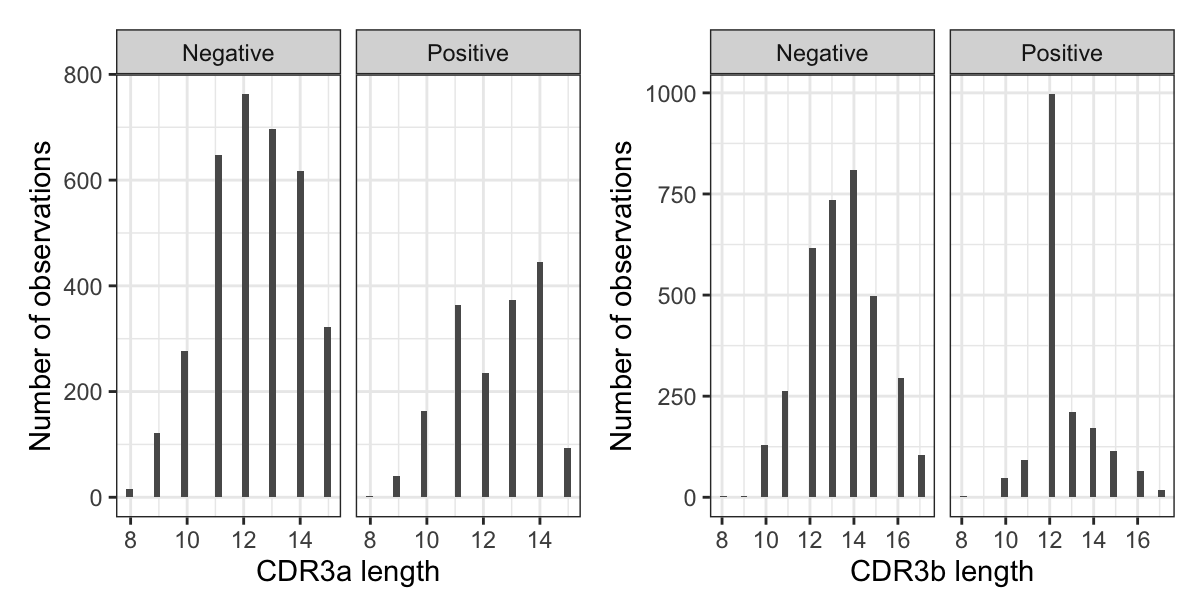
\includegraphics[width = \linewidth]{figures/cdr3_lengths.png}
    \caption{CDR3 lengths for 10x negative and positive TCRs.}
    \label{fig:cdr3_length}
\end{figure}

\begin{figure}
    \centering
    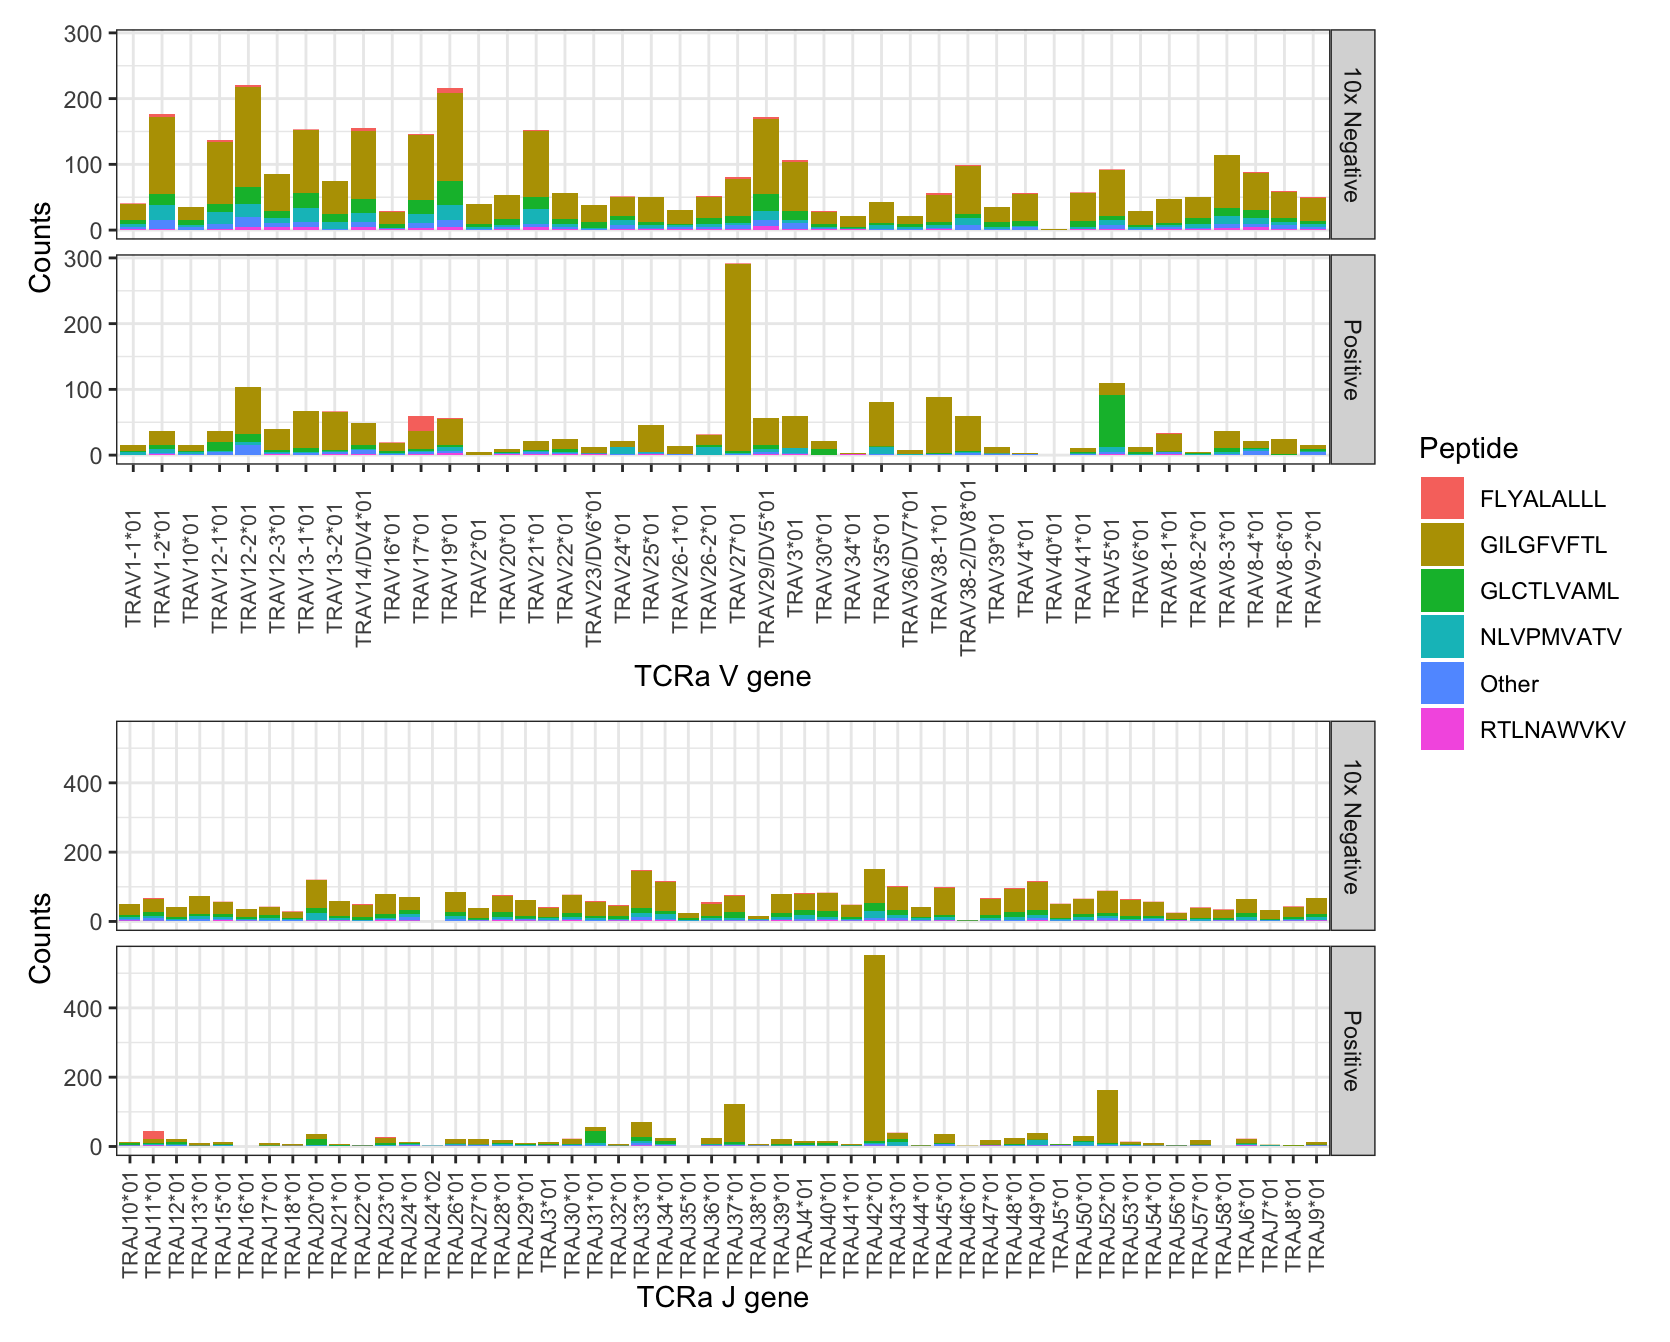
\includegraphics[width=\linewidth]{figures/tcra_genes.png}
    \caption{Germline genes used in the TCR{\textalpha} sequences in the data.}
    \label{fig:tcra_genes}
\end{figure}

\begin{figure}
    \centering
    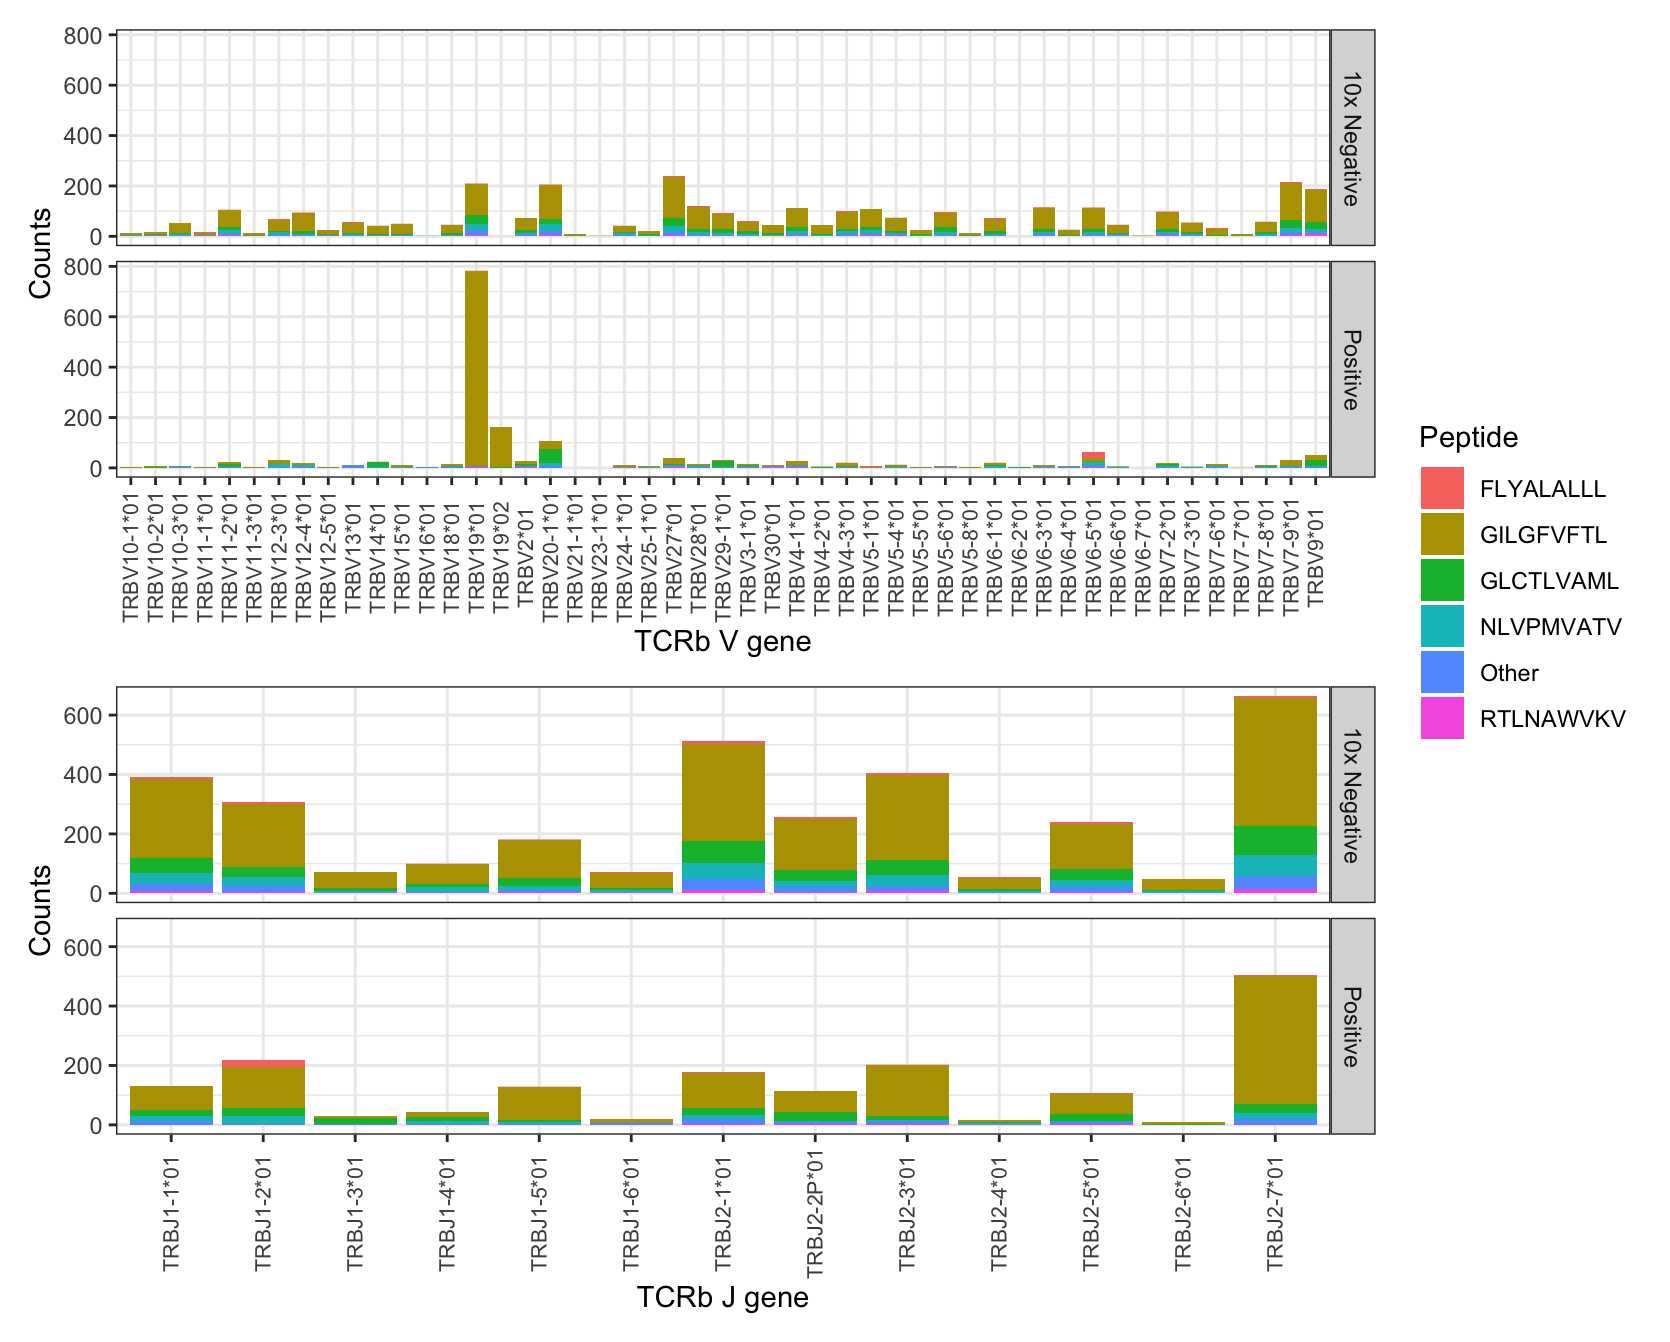
\includegraphics[width=\linewidth]{figures/tcrb_genes.png}
    \caption{Germline genes used in the TCR{\textbeta} sequences in the data.}
    \label{fig:tcrb_genes}
\end{figure}
\clearpage
There are 18 unique peptides in the dataset, which have a large span in terms of the number of observations. The number of observations per peptide is shown in Figure \ref{fig:obs_per_pep}. The 10 most frequent peptides are displayed stratified on their origin. There is a clear bias for the GILGFVFTL (GIL) peptide in the positives, with 1233 out of 1718 positives. Because we preserve the ratio between positives and negatives across peptides, there is also a large bias in the negatives towards GIL. 


\begin{figure}[H]
    \centering
    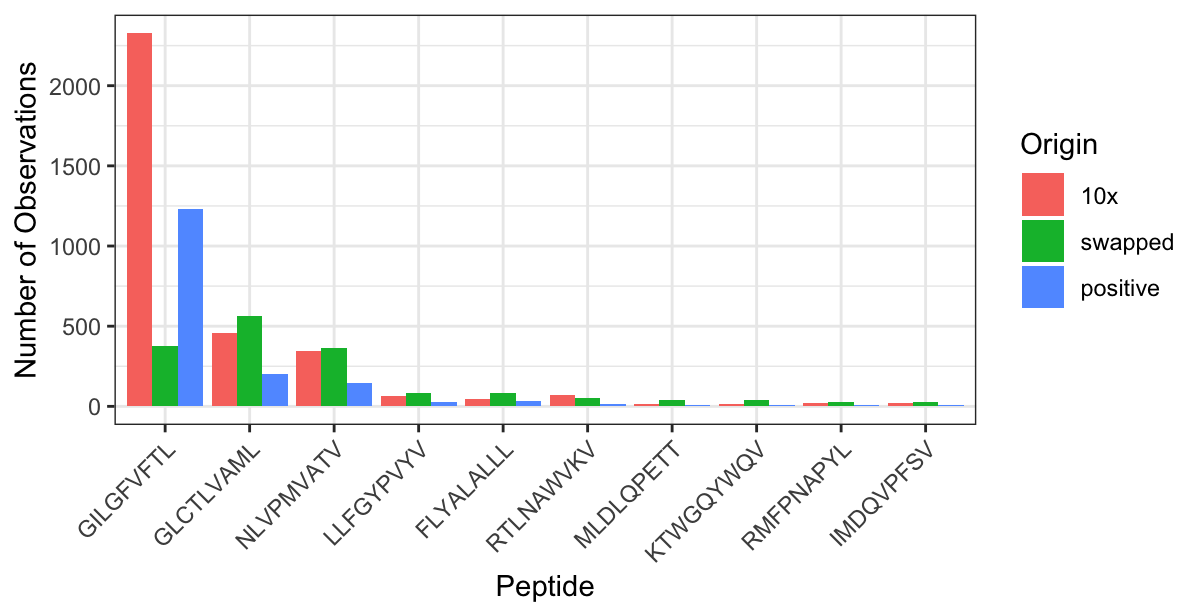
\includegraphics[width = \linewidth]{figures/Observations_per_peptide.png}
    \caption{Number of observations per peptide and origin for the 10 most frequent peptides.}
    \label{fig:obs_per_pep}
\end{figure}

The swapped peptides have a different distribution than the other types of observations. Here a random peptide was chosen from positive observations with other peptides. Since most positive observations are positive for GIL, a TCR positive for the GLCTLVAML (GLC) peptide will often be observed as a swapped negative with the GIL peptide. If the swapped peptide was chosen from a unique list of peptides, there would rarely be any swapped observations with a GIL peptide since most positive observations are from GIL. By choosing a random peptide from the dataset, the swapped peptides have a distribution more like the rest of the data compared to creating swapped from a unique list.

The bias in the peptides can affect the pan-specific models' ability to predict infrequent peptides in the dataset since the signal from these observations is overshadowed by much more frequent peptides such as the GIL peptide.

\subsection{Locating important features for model performance}
It is unreasonable to assume all sections of the TCR are equally important for recognition of the pMHC complex, as the CDRs are much closer to the displayed peptide than the framework regions on the TCR (Figure \ref{fig:tcr_xray}). Therefore, we investigated which areas of the sequence were required for performance and which features were the most substantial for TCR-pMHC binding predictions. The CNN model was trained on varying amounts of input by leaving out either different sequences and features.

Figure \ref{fig:reduce_input} shows the AUCs for these experiments.  The TCR and peptide are needed in some capacity to achieve meaningful performance in most cases. Removing the peptide restricts the model to distinguish between positive and negative TCRs in general instead of distinguishing at a peptide-specific level, which results in a performance drop. Removing the MHC has no real effect on performance and, in most cases, achieves the same or better performance. This is unsurprising, as the data used here only contains HLA-A02*01. The input does not add any information and the higher number of parameters most likely leads to overfitting for models containing the MHC. Restricting the TCR to only the CDR3s gives the same or a slightly increased performance in all cases except for only energy features. This supports the idea that the CDR3s are the most important parts of the sequence for determining TCR specificity \cite{Glanville2017IdentifyingRepertoire, Wong2019ComparativeReceptors}. 

Interestingly, using only the energy features as input allows models trained even without the TCR to recover some performance. The most likely explanation to this is that large interaction energies increase binding probability. It thereby gets some information about the TCR through the interaction energies between the TCR and peptide.

Often the most interesting model is also the simplest model. Feature selection was done by first evaluating the significance of the top-performing model for each type of feature input and selecting the simplest model of the significantly best performing models. Afterwards, all models from that feature type were tested against each other, and the simplest model of the significantly best performing models was chosen. 

When selecting the most important features, the model with only energy features was significantly worse than all other models (P < 0.05 for all tests using bootstrapping with 10000 replications), while all other models were equivalent. For selecting the most important sequence, the model with only peptide and CDR3 is significantly better than all other models (P < 0.05 for all tests using bootstrapping with 10000 replications). Therefore, we focus on training models using only the sequence features for the peptide and CDR3s for the remainder of this thesis.

\begin{figure}[H]
    \centering
    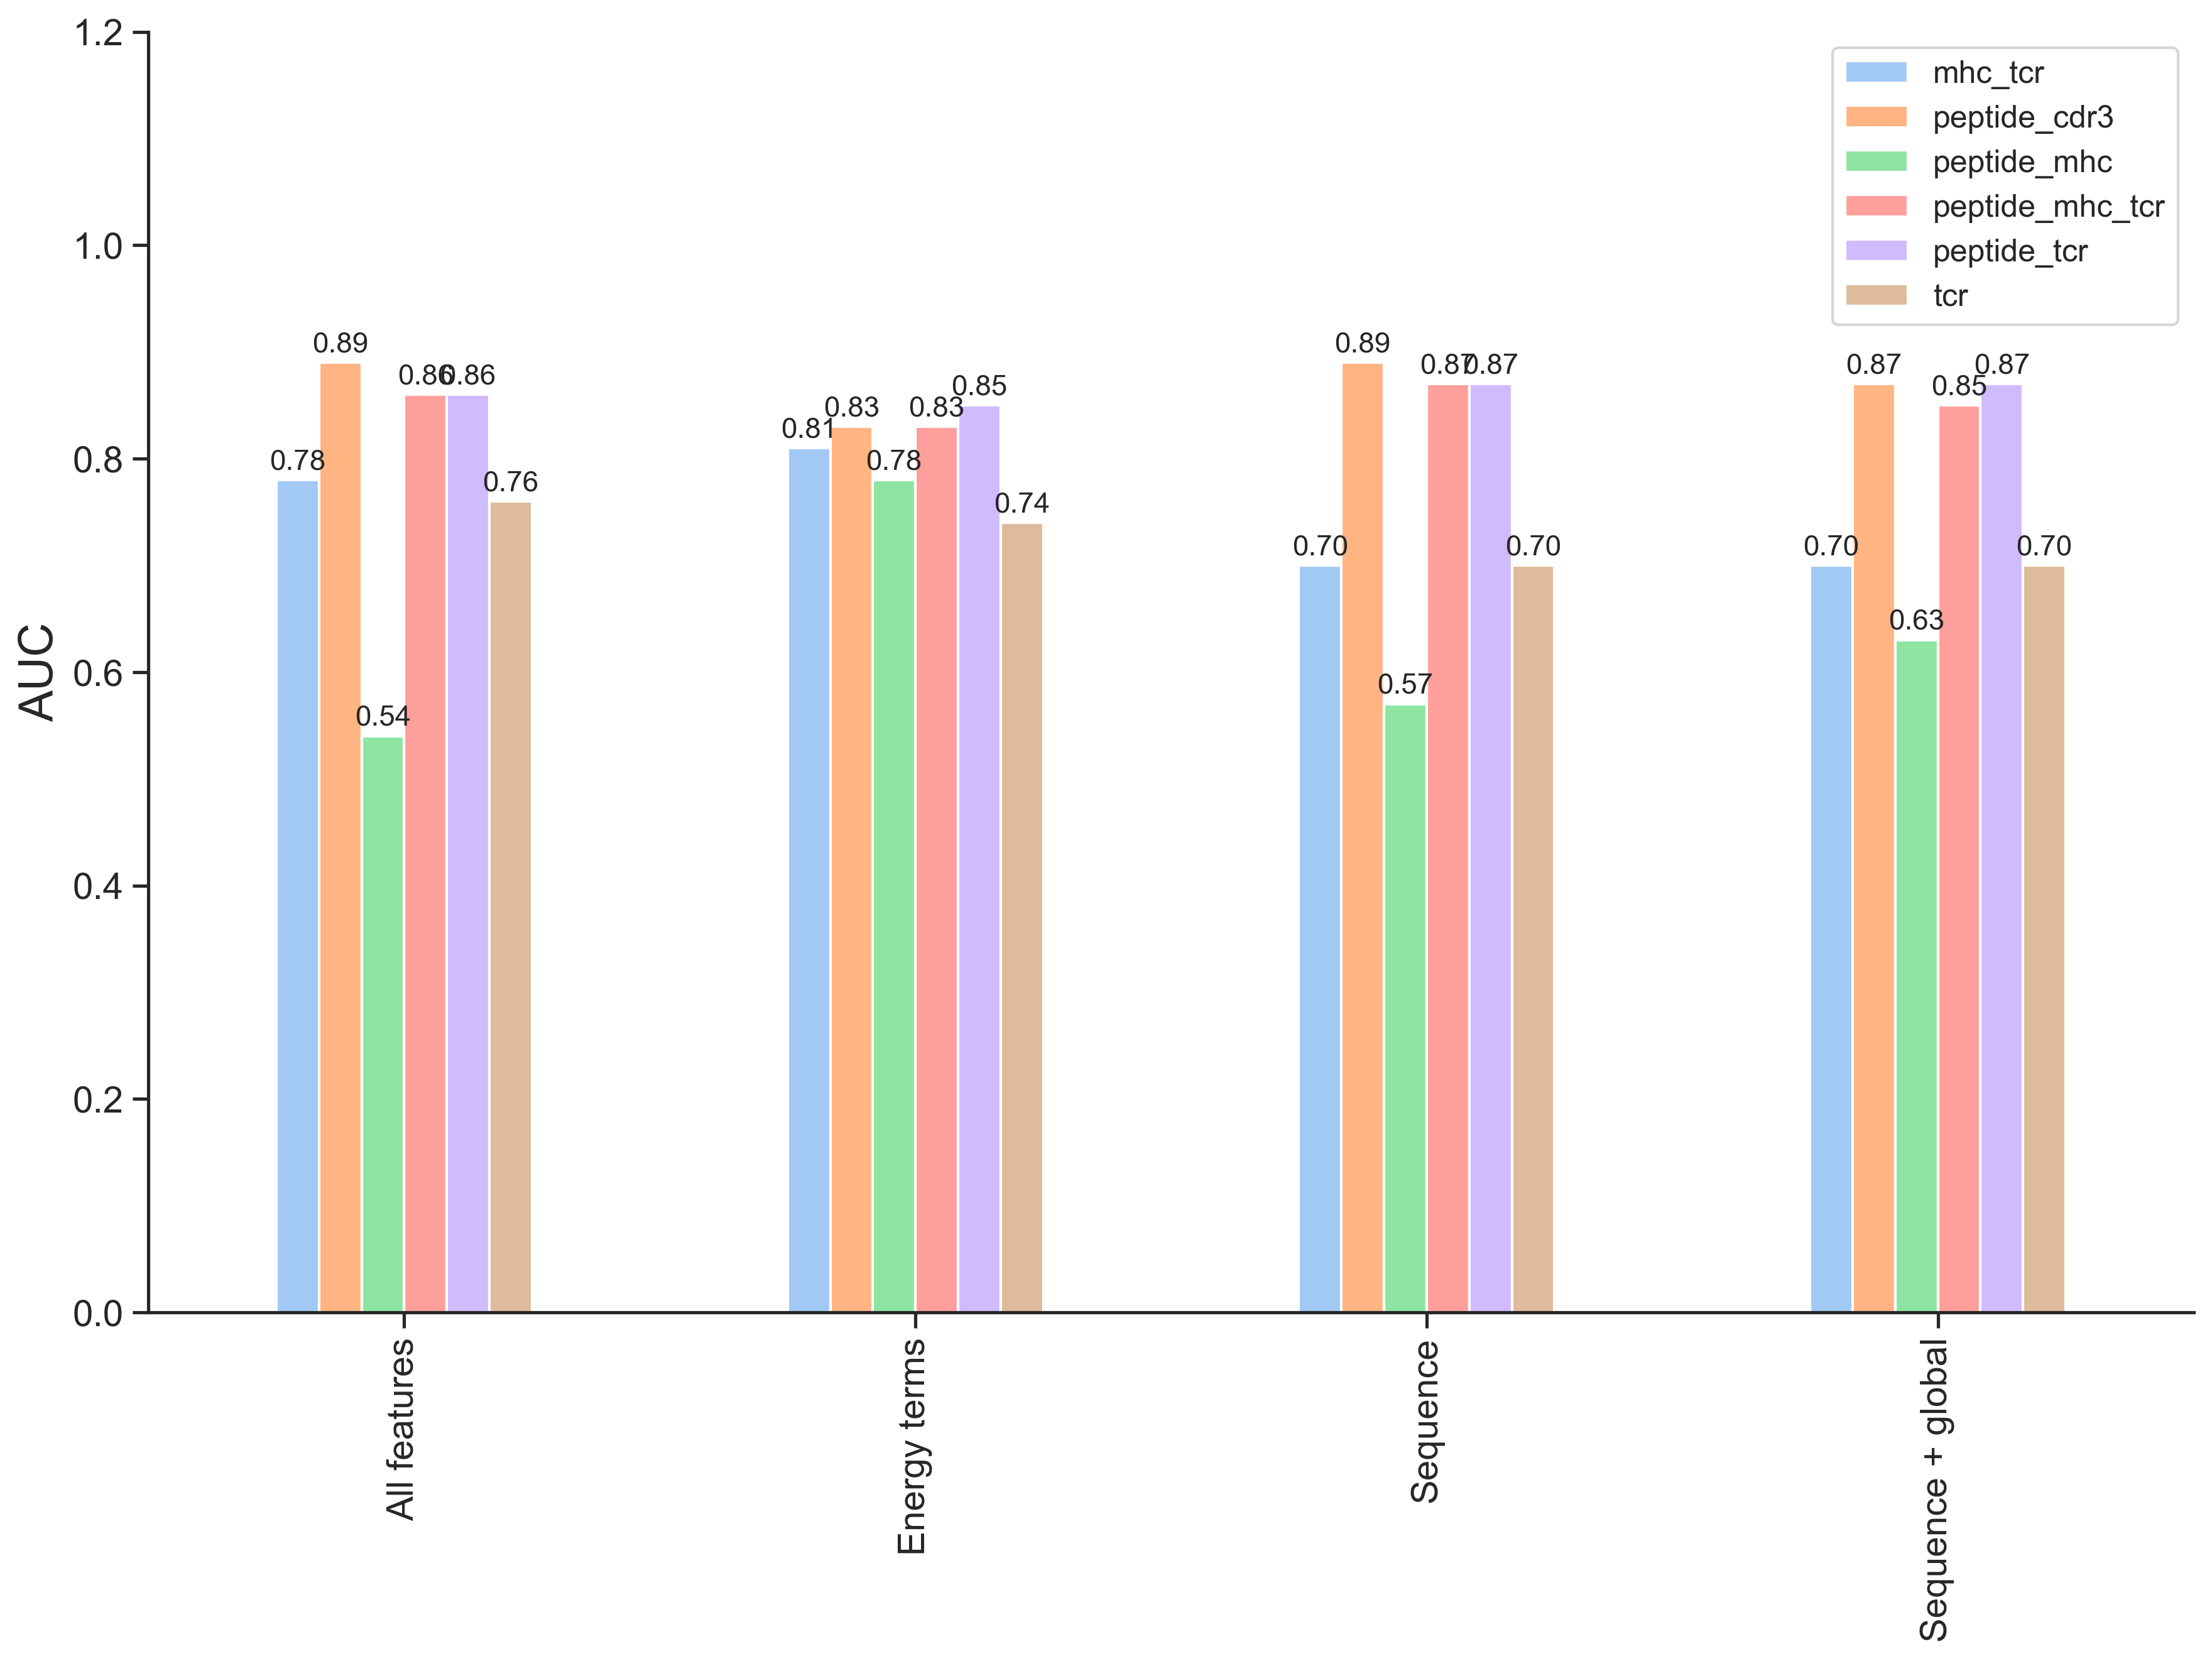
\includegraphics[width=\linewidth]{figures/reduce_input.png}
    \caption{AUC for the CNN model trained on different amounts of input. AUC was evaluated using nested cross-validation. All features refers to using sequence, per-residue energy features and global energy features. The energy terms are only trained on per-residue and global energy features. Sequence is trained on only the sequence encoding. Sequence + global leaves out the per-residue energy features. These features were then trained with different number of sequences. The legend describes the types of sequences used in that model.}
    \label{fig:reduce_input}
\end{figure}

Paired CDR3{\textalpha} and CDR3{\textbeta} data is more expensive than bulk sequencing of only the CDR3{\textbeta}. We investigated whether a paired model performs better than models trained only on CDR3{\textalpha} or CDR3{\textbeta}. CNN models were trained on the same data using the peptide and either both or only one of the CDR3 sequences. As seen in Figure \ref{fig:cdrab_vs_a_b}, the paired CDR3 approach obtains a score of 0.88, compared to 0.81 and 0.83 for the CDR3{\textalpha} and CDR3{\textbeta} respectively. The difference between the paired model and the individual sequence is significant (P < 0.05 using bootstrapping with 10000 replications). In contrast, the difference between the two individual models is not significant (P = 0.42 using bootstrapping with 10000 replications). 

Both chains seem to be important for generating accurate TCR-pMHC binding predictions. While the model using only the CDR3{\textbeta} does slightly outperform the CDR3{\textalpha}, there was no significant difference between the two. Thereby we have reduced the input space for the model from having MHC, peptide and the entire TCRs represented by both a sequence encoding and predicted energy features to include the peptide and CDR3s from the TCRs represented by a sequence encoding.

\begin{figure}[H]
    \centering
    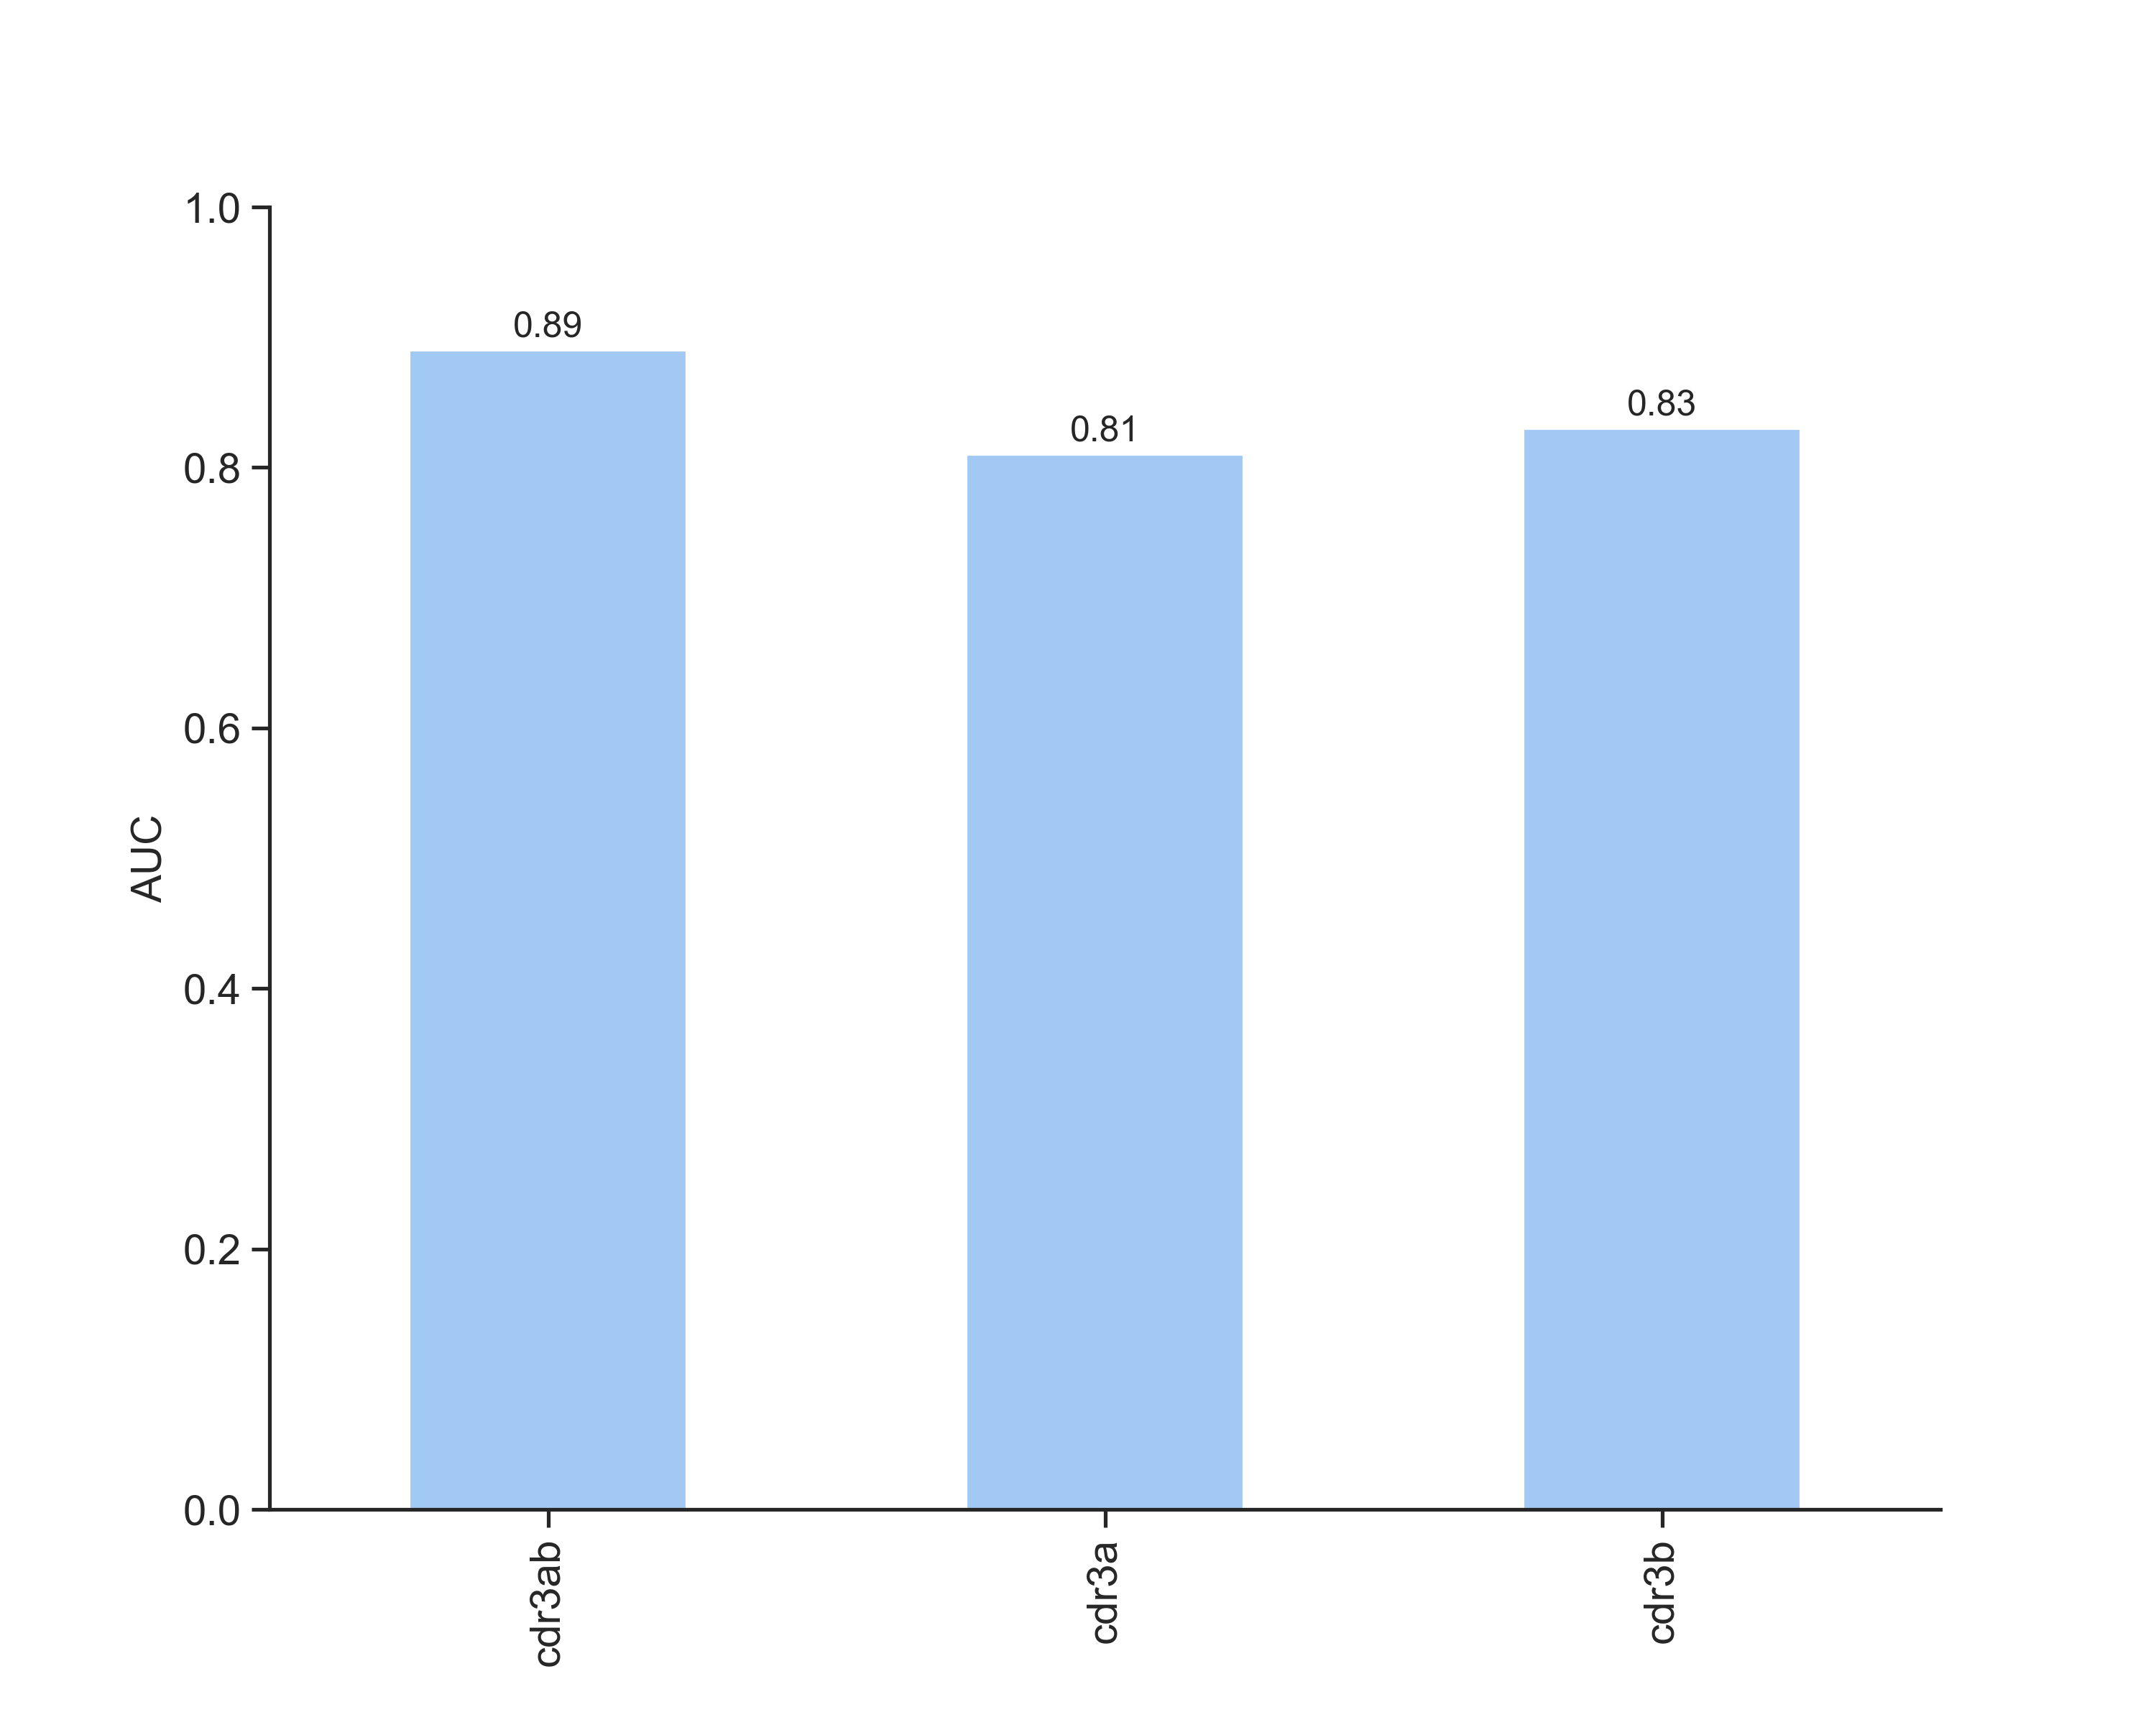
\includegraphics[width=0.75\linewidth]{figures/cdr3ab_vs_a_vs_b.png}
    \caption{AUC for CNN models trained on both chains (cdr3ab) or single chains. AUC was calculated using nested cross-validation.}
    \label{fig:cdrab_vs_a_b}
\end{figure}

\subsection{Attention Mechanisms Focuses On Residues Specific For Positives}
This section describes which areas of the CDR3s the model chooses to focus on and investigate if there is any relationship to differences between positive and negative sequences.

\subsubsection{Positions Selected By CNN Maxpooling}
CNN based models have previously been used for predictions of TCR-pMHC interactions \cite{IsabellJurtz2018NetTCR:Networks, Montemurro2021NetTCR-2.0Data}. The CNN models contain a max pooling operation, which allows the network to select the most important positions for predicting T cell interactions, and also allows the model to disregard specific areas on the sequence. The positions selected from filters might provide insight into important positions used to identify positive TCRs and how the model determines what should be classified as positive and negative.

As mentioned in Section \ref{cnn}, the convolution operation incorporates information from adjacent positions (For this model, three positions). The max pooling operation then selects a single convoluted value by selecting the maximum value. Each filter in the network represents information about three of the original positions used to create the convolutional output value. The number of times a filter selects a specific position can therefore be used to evaluate how important each position is relative to other positions in that sequence.

The counts for each position can be seen in Figure \ref{fig:pool_gil12a} for CDR3{\textalpha} and Figure \ref{fig:pool_gil12b} for CDR3{\textbeta}. The figures show CDR3s that were either positive (graph 1) or 10x negative (graph 3) towards GIL. As the filters used has size 3, each position is convoluted three times and can be selected at three different positions. The first and last two positions are convoluted only once or twice. Therefore, it is expected that these positions will have lower counts than others. There is, however, a clear difference in what the important regions for the CDR3{\textalpha} and the CDR3{\textbeta} are. The CDR3{\textbeta} primarily focuses on positions 4-7, while the CDR3{\textalpha} has no enrichment, except for a slight increase for positions 9 and 10. However, no clear distinction can be made between the positives and 10x negatives for either CDR3s. There are slightly more counts at positions 8 and 9 for the 10x negative CDR3{\textbeta} relatively to the same positions for the positive CDR3{\textbeta}.

The model contains many filters, and some of these filters might contribute noise or only a little information for making predictions. The convolution value is passed through the sigmoid function before max pooling. Since the sigmoid squishes values to the interval $(0 , 1)$, then large values will have a bigger impact in the dense network, and are therefore deemed more important by the network. Unimportant filters can therefore be removed by only counting convolutions whose value is larger than a threshold (0.9) When comparing the number of filters per position without setting a threshold (graphs 1 and 3) to with a threshold (graphs 2 and 4), the most substantial change can be seen on the CDR3{\textalpha}. Here, there is a larger enrichment at positions 9-11 than without the threshold. The counts for the CDR3{\textbeta} with threshold are similar to without, except for a drop at position 8. For both CDR3s, the model has learned which sections contain padding (positions 13 and up) and actual information. The number of filters placed in the padding is substantially smaller with a threshold than without the threshold. Filters that sit in the padding likely have a low influence on the prediction due to the low activation value it carries over into the dense layers. The same analysis was performed on NLVPMVATV (NLV), with similar results (Appendix A).

The model has learned to focus on areas with information and learned to limit the information from padding. However, there was no clear distinction between positions chosen for positives and negatives. Therefore binding probability might be determined by differences in residues at these positions or interactions between individual filters in the hidden layer.

\begin{figure}[H]
\centering
\begin{subfigure}[b]{0.7\textwidth}
   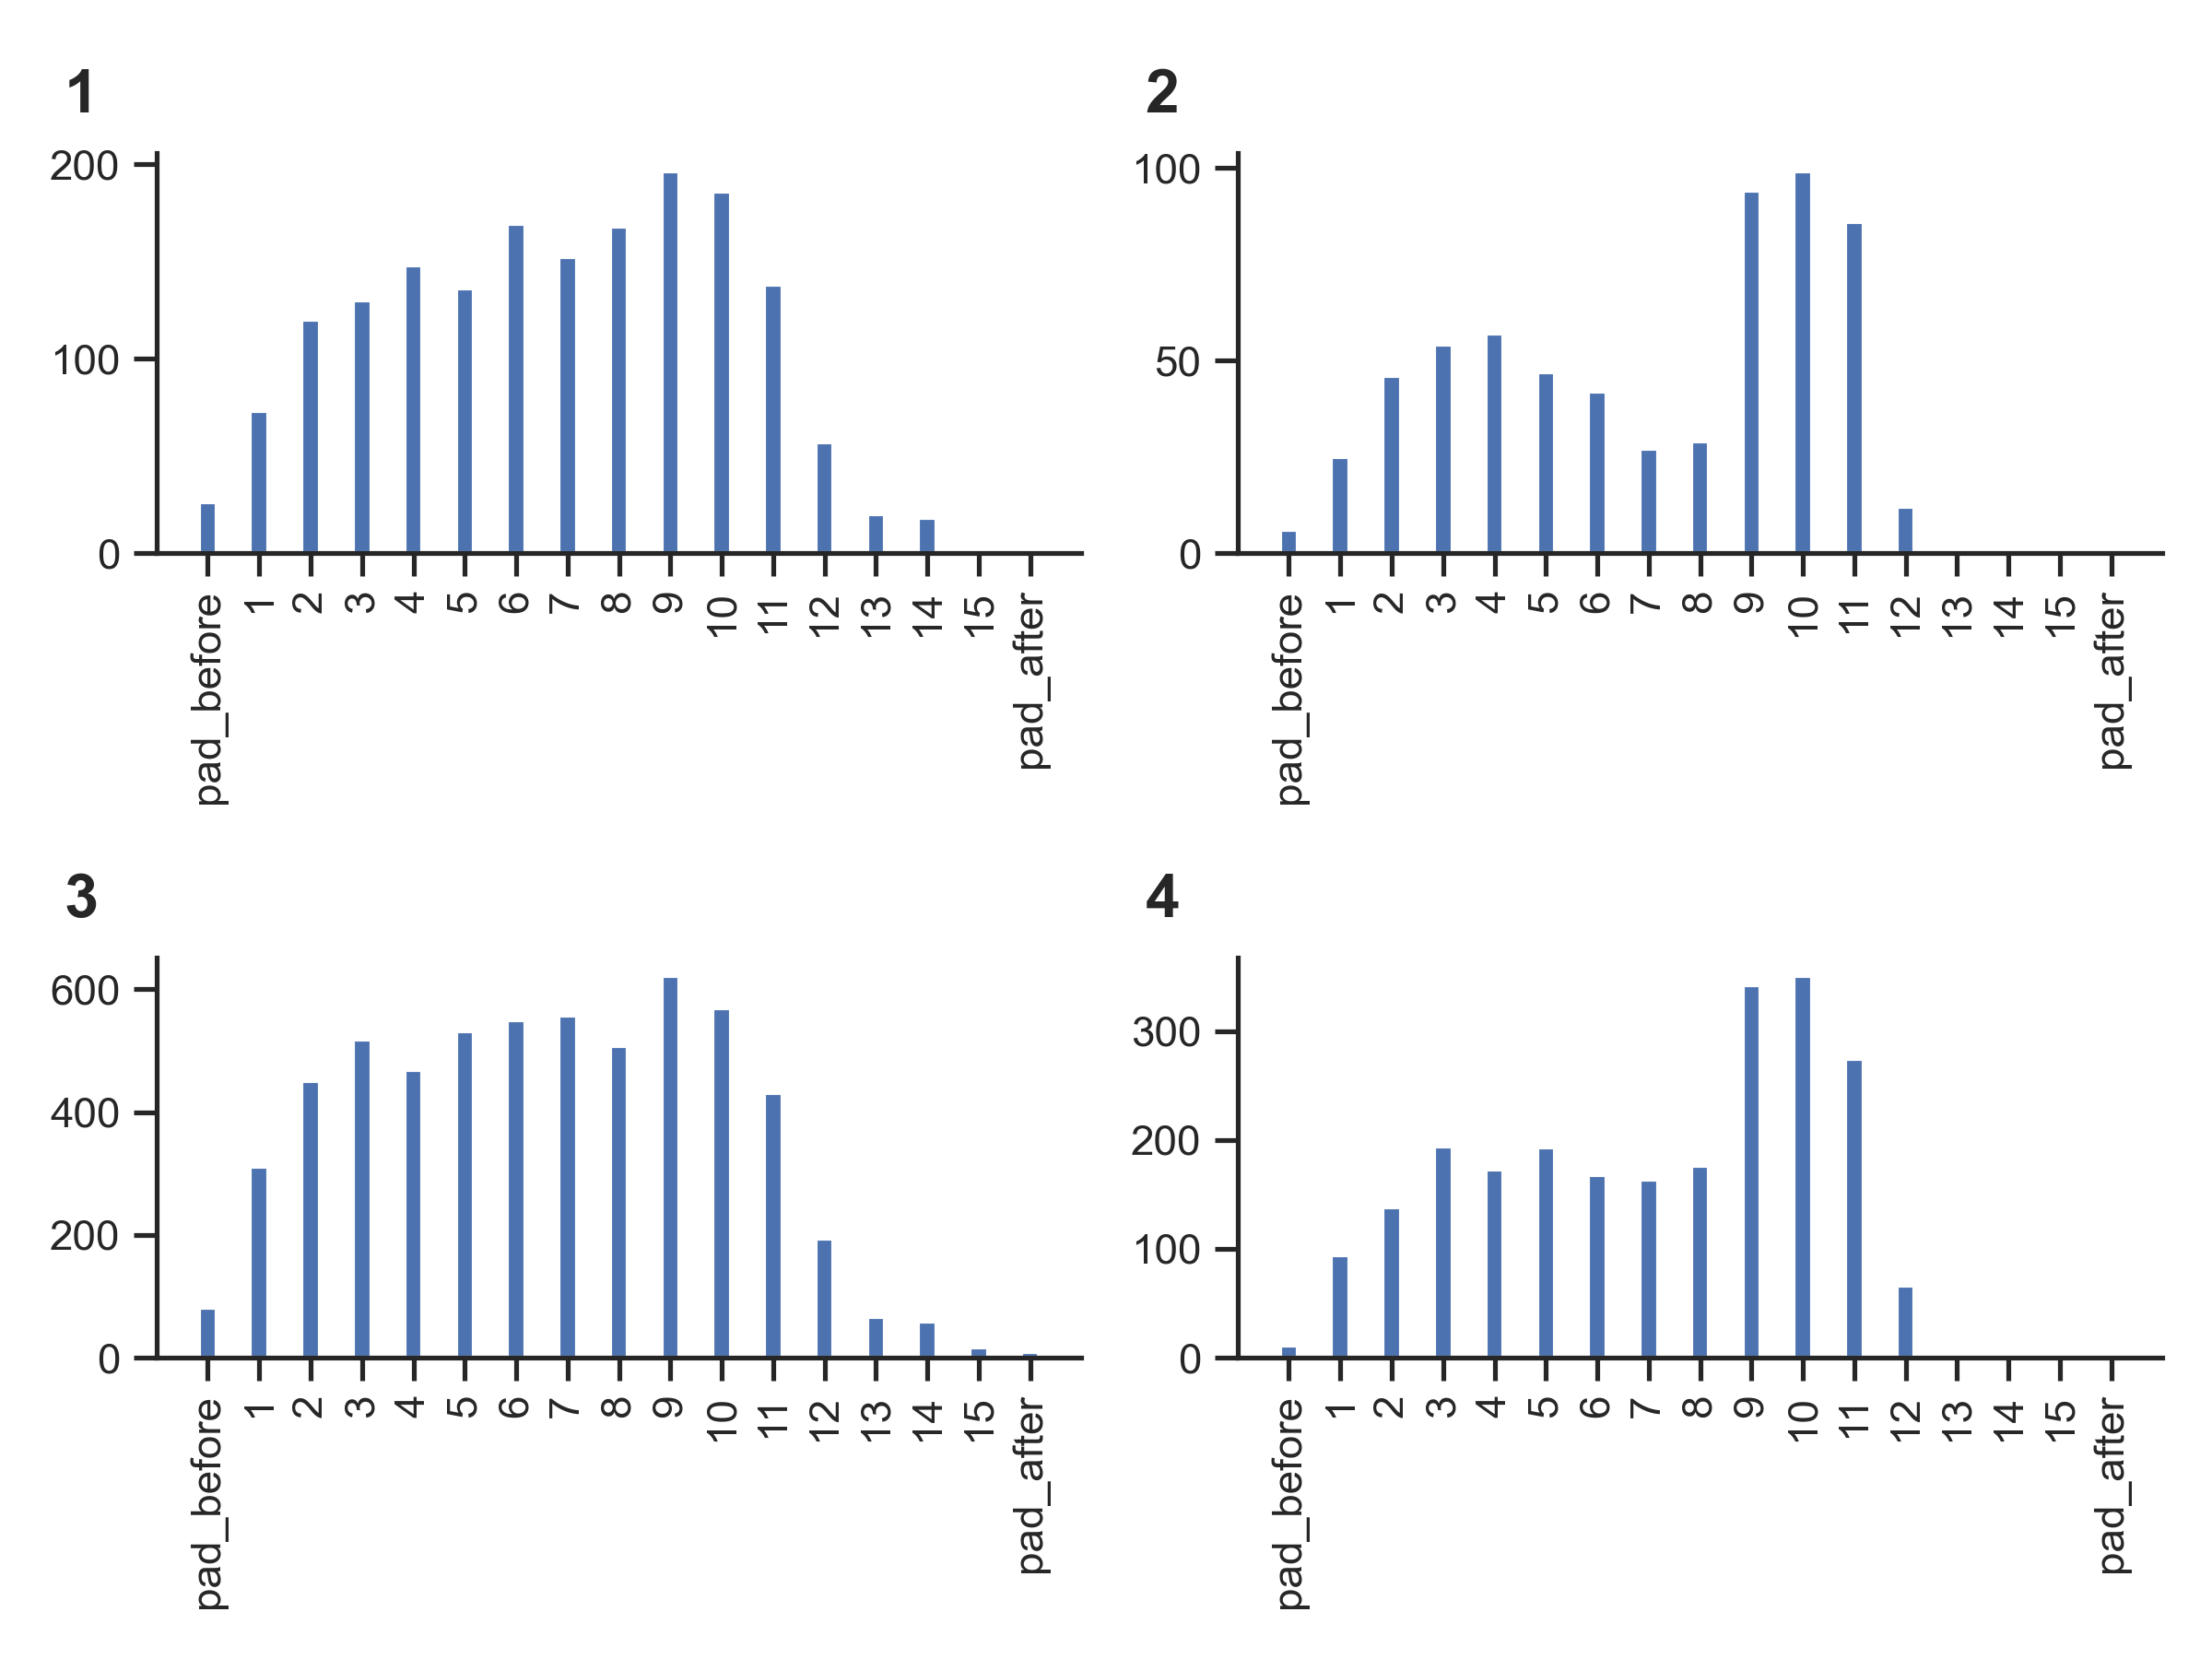
\includegraphics[width=1\linewidth]{figures/attention_results/maxpool_cdr3a_gil12.png}
   \caption{Histograms for CDR3{\textalpha}.}
   \label{fig:pool_gil12a} 
\end{subfigure}

\begin{subfigure}[b]{0.7\textwidth}
   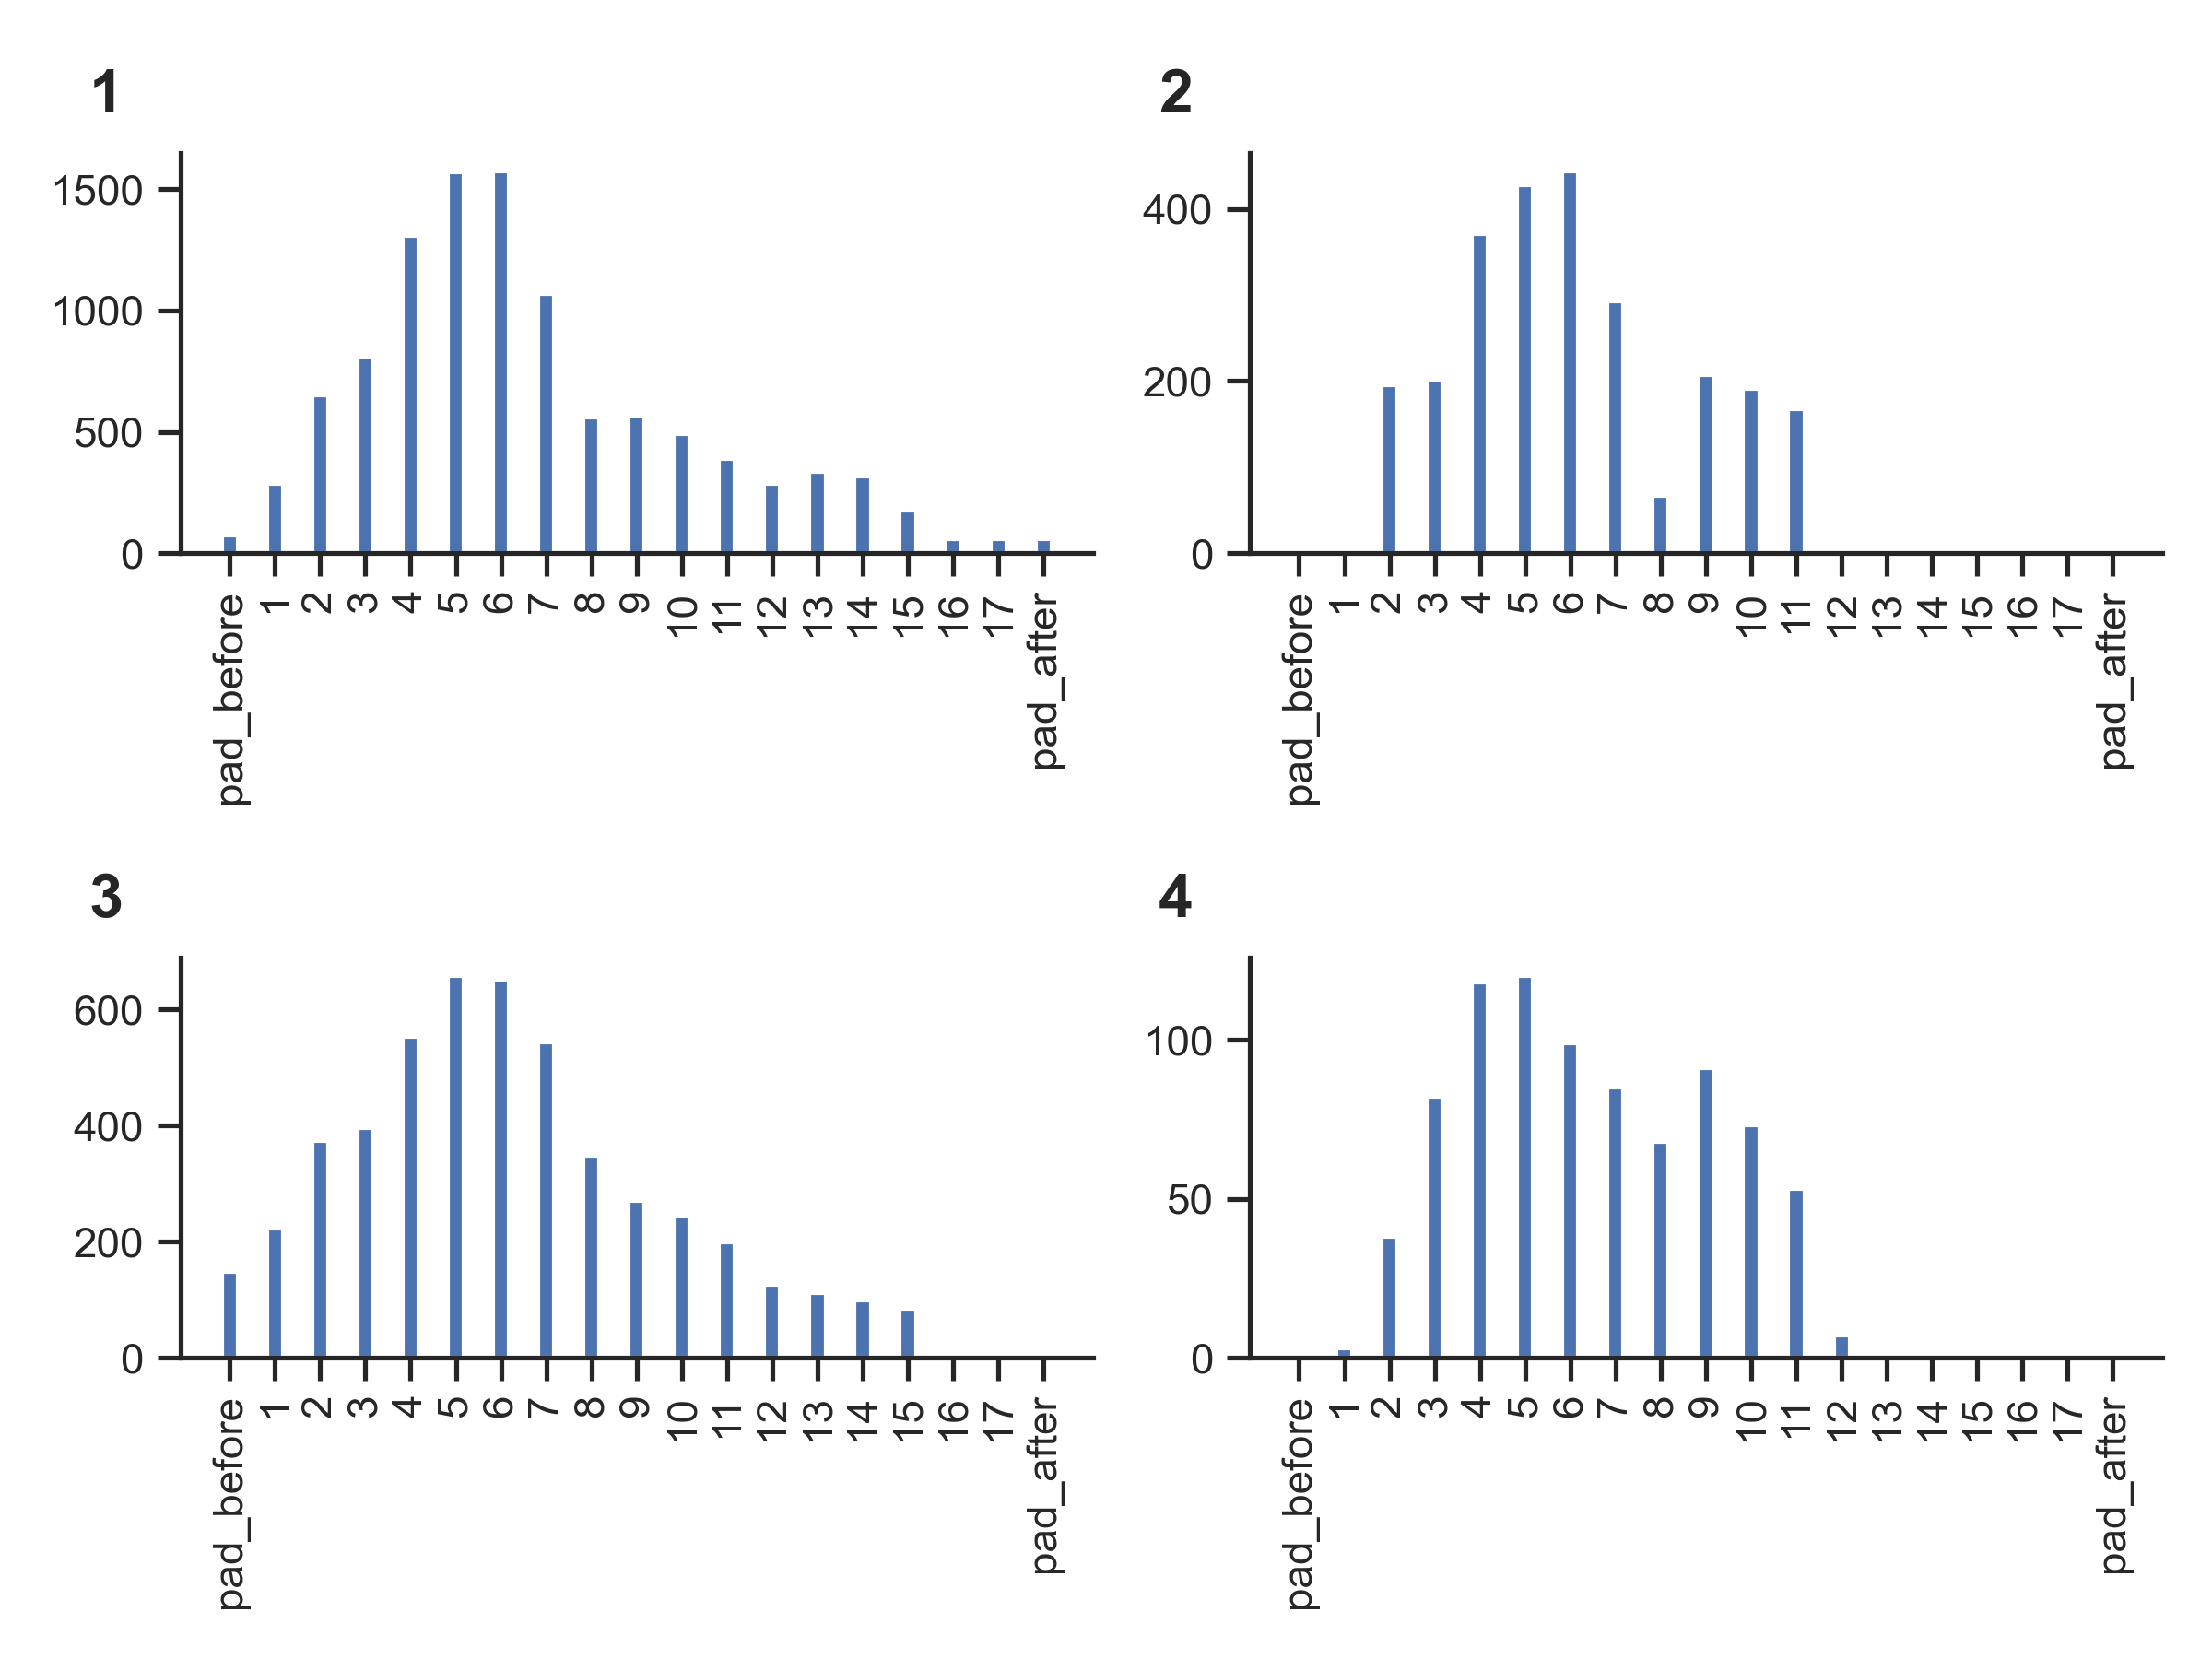
\includegraphics[width=1\linewidth]{figures/attention_results/maxpool_cdr3b_gil12.png}
   \caption{Histograms for CDR3{\textbeta}.}
   \label{fig:pool_gil12b}
\end{subfigure}
\caption{Histograms of the number of times a position is selected to contribute information by the max pooling operation. Positions are considered contributing if they are used in the convolution selected by max pooling. \textbf{(1)} Positions selected for CDR3s with positive interaction. \textbf{(2)} As (1), but only considering filters with an activation above 0.9 \textbf{(3)} Positions selected for negative CDR3s from the 10x dataset. \textbf{(4)} As (3), but only considering filters with an activation above 0.9. Data shown for partition held out during training limited to CDR3{\textalpha} and CDR3{\textbeta} with length 14 and 12 respectively and specificity for GIL.}
\end{figure}

\subsubsection{Positional Attention On biLSTM Positions}
While max pooling a convoluted sequence can be regarded as attention, the attention is learned purely based on the weights inside the convolutional filters. Instead, the attLSTM model uses a learnable weight vector and matrix to calculate the most important positions. It can incorporate information from multiple areas of the sequence using a single context vector, whereas max pooling only transfers information about 3 adjacent residues.

The capabilities of the attention mechanism was shown by training The attLSTM  using TCRs instead of CDR3s. The positional attention for each positive sequence is shown in Figure \ref{fig:att_tcrs}. We expect to find the attention primarily on areas important for binding predictions, and it should ignore other areas. For the TCR{\textalpha} the attention on the sequences is almost contained to the CDR3, with 48\% of the attention being put on the CDR3. This percentage is much higher than the 15\% expected for a uniform attention across the entire sequence. For the TCR{\textbeta} the attention is more spread, and some attention is put on framework regions that are unlikely to have importance for binding. However, there is still a clear tendency to focus on the CDR3, which contains 25\% of the attention in contrast to the expected 15\% for uniform attention. The noise is perhaps due to a large germline bias in the positive CDR3 observations (Figure \ref{fig:tcra_genes}-\ref{fig:tcrb_genes}), which might allow the model to learn positives purely based on conserved areas in the framework regions for that germline. Therefore, attention allows the model to capture information from the areas in the sequence known to be important for binding \cite{Tsuchiya2016TheLoops}.

\begin{figure}[H]
    \centering
    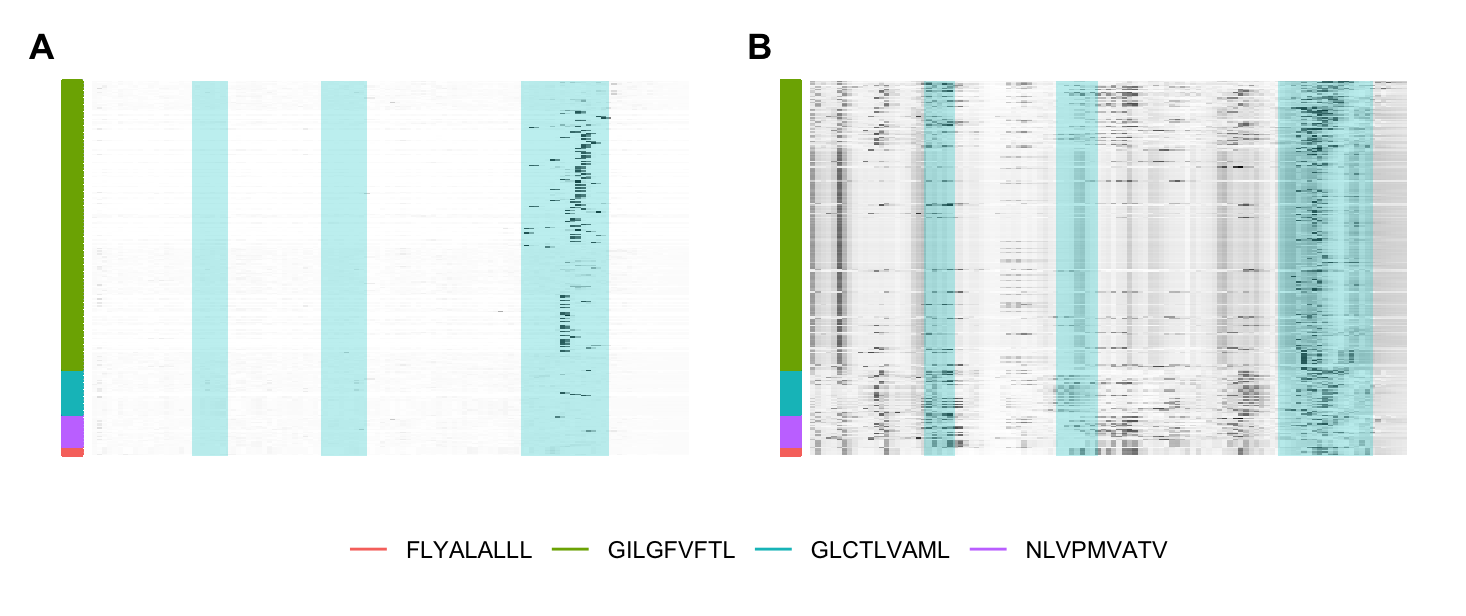
\includegraphics[width=\linewidth]{figures/attention_results/att_tcrs.png}
    \caption{Importance of positions for generating the weighted hidden state for the forward direction of positive \textbf{(A)} TCR{\textalpha} and \textbf{(B)} TCR{\textbeta}. Blue annotations reflect approximate positions of CDRs. Data shown for partition held out during training.}
    \label{fig:att_tcrs}
\end{figure}

The approach was then applied only CDR3s to locate important positions in the CDR3s, and see if there were any similarities to the results found for the CNN model.

The attention vectors for positive and negative CDR3{\textalpha} and CDR3{\textbeta} is plotted in Figure \ref{fig:att_cdrs}. The positive CDR3{\textalpha} (Figure \ref{fig:att_cdrs}A) has a clear pattern in the sequences specific for GIL, where the model focuses around position 11-12 for the longest sequences (length 14). Since sequences have been padded to the same length on the right, the positions focused by the attention are located at the same relative position in the sequence. These positions may therefore be important for discriminating between positives and negatives for GIL. The pattern for CDR3{\textalpha}s is less clear on peptides other than GIL The attention is more spread and does not contain the same length-dependent pattern. When that is said, some sequences seem to have a preference for position eight in some manner. The length-dependent pattern cannot be recovered for any of the peptides for the negatives. Instead, there is some preference for the first position, which is also seen in some of the positive observations. The explanation for this could be that the attention layer primarily looks for motifs in positive sequences, and something more arbitrary is chosen if these motifs cannot be found. The first position is unlikely to provide much information as it is fairly conserved for all sequences. 

The length-dependent pattern indicates that CDR3{\textalpha}s positive for GIL have some motif in the latter part of the sequence not found in the negatives. The GIL's clear pattern and absence in other peptides could indicate overfitting to the GIL peptide, which would not be surprising, as most of the data is specific for this peptide.

The positive CDR3{\textbeta} also contains the length-dependent pattern (Figure \ref{fig:att_cdrs}C). However, for a large number of the positive sequences, the attention is primarily focused on positions 6 and 7. These are CDRs with length 12, and have a large germline bias (Figure \ref{fig:cdr3_length}-\ref{fig:tcrb_genes}). Compared to the CDR3{\textalpha}, where the length-dependent did not repeat for peptides other than GIL, the CDR3{\textbeta} has the same pattern reappearing in the less frequent peptide as well. This could mean the learned attention is more general than for the CDR3{\textalpha} and that these positions are important for peptide binding predictions for more than just GIL. The negative CDR3{\textbeta} similarly has a (Figure \ref{fig:att_cdrs}D) length-dependent pattern. The positions selected by attention are roughly the same for positive and negative CDR3{\textbeta}. The difference in the plots is due to differences in length distributions (Figure \ref{fig:cdr3_length}), as the positives have a huge overweight of peptides of length 12.

Attention on the CDR3{\textbeta} seems to capture some signal at the middle of the sequence, and these positions carry most of the information required. The strong attention put on specific positions for peptides with a length of 12 could point towards the model overfitting or finding biological relevant residues for predictions on these peptides. These constitute a large section of the positive dataset, whereas noticeably fewer of the corresponding negative CDR3{\textbeta}s with length 12 exist. This indicates that the model is learning some of the dataset's bias. Therefore, even though there is clear attention at positions 6 and 7, it is probably not a general way to discriminate between positives and negatives TCRs.
The attention of the reverse directions was more unstable between runs and contained a lot of noise (Appendix B). Training the model without the reverse LSTMs also gave comparable results to training it as a biLSTM (not shown). The model, therefore, seems to get most of its information from the forward directions, and the reverse directions do not contribute much, which could explain the high levels of noise and unclear patterns in the attention vector.

\begin{figure}[H]
    \centering
    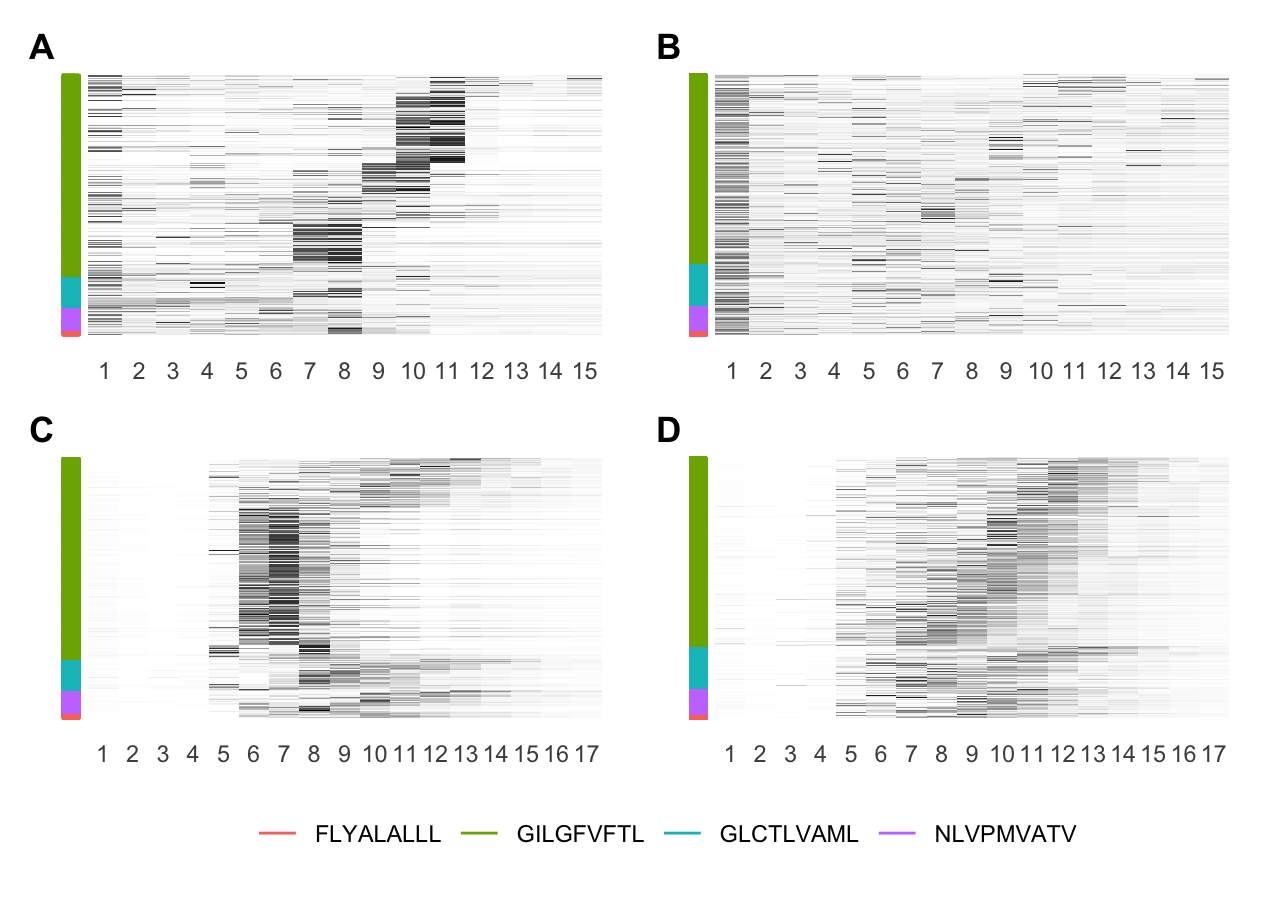
\includegraphics[width=\linewidth]{figures/attention_results/att_cdr3s.png}
    \caption{Attention on positions for generating the weighted hidden state for the forward direction of \textbf{(A)} Positive CDR3{\textalpha}, \textbf{(B)} Negative CDR3{\textalpha}, \textbf{(C)} Positive CDR3{\textbeta} and \textbf{(D)} Negative CDR3{\textbeta}. Sequences have been sorted by CDR length in descending order. Data shown for partition held out during training.}
    \label{fig:att_cdrs}
\end{figure}

\subsubsection{Sequence Logos For CDR3s}
The positions with strong attention may contain specific motifs in the sequence, which the model focuses on and uses to distinguish between positives and negatives. The attention vectors (Figure \ref{fig:att_cdrs}) could be indicating where these positions are located. A sequence logo was generated for both positive and negative CDR3{\textalpha} of length 14 and CDR3{\textbeta} of length 12 to see if the attention patterns correspond to differences in the motifs. The attention for CDR3{\textalpha} of length 14 primarily focuses on positions 10 and 11, while attention for CDR3{\textbeta} with length 12 mostly focuses on positions 6 and 7 (Figure \ref{fig:att_cdrs}). 

Comparing the logos for CDR3{\textalpha} with length 14 (Figure \ref{fig:logo_cdr3apos} and Figure \ref{fig:logo_cdr3aneg}) shows that generally glycines are more conserved in the central positions for both the positive and negatives. The positions 9, 10 and 11 seem to differ the most between the two logos and concur with the difference observed between the two attention vectors for CDR3{\textalpha} sequences with length 14. The motif QGN is present in the positives but not in the negatives. Especially the glycine is quite conserved at position 10 and not present for the negatives. Other positions, while more conserved in the positives, are also present in the negative logo.

Logos for GIL positive CDR3{\textalpha} with lengths 13 and 11 (Appendix C) has the same motif as found in sequences of length 14. However, the position of the motif has moved due to the shorter length, as the length-dependent pattern indicated in Figure \ref{fig:att_cdrs}. In these logos, the over-represented glycine instead resides in position 7 or 9 and the asparagine in position 8 or 10 for the 11 and 13 long CDR3{\textalpha}. The QGN motif is a central part of the TRAJ:42*01 gene, meaning this is not part of junction residues, but a result of gene bias present in the data.

The logos for CDR3{\textbeta} with length 12 primarily differs in arginine and serine present in the positive logo (Figure \ref{fig:logo_cdr3bpos}), but not present in the negative logo (Figure \ref{fig:logo_cdr3bneg}). However, these differences are located at positions 5 and 6 and do not line up completely with the results found in Figure \ref{fig:att_cdrs}, where the focus was primarily on positions 6 and 7. Instead, it lines up with the results seen for the CNN model (Figure \ref{fig:pool_gil12b}). Why this occurs is unknown, but the LSTM might pass the information from the input at positions 5 and 6 to position 7 through the hidden and cell state passed to position 7, where the attention mechanism captures the signal.

The attention vectors have learned some of the key differences in the sequence between the positive and negative CDRs. The QGN motif in the CDR3{\textalpha} is a central part of the discrimination between positive and negative for GIL. The motif is a part of TRAJ:42*01 and is therefore not limited to a single length but can be found in sequences with multiple lengths as seed by the attention vectors (Figure \ref{fig:att_cdrs}). For the CDR3{\textbeta} the model either passes the information about the sequence to the next position in the LSTM and incorporates it there or learns to differentiate in a more complex manner not captured by the sequence logos.

\begin{figure}[H]
\centering
\begin{subfigure}[b]{0.45\textwidth}
   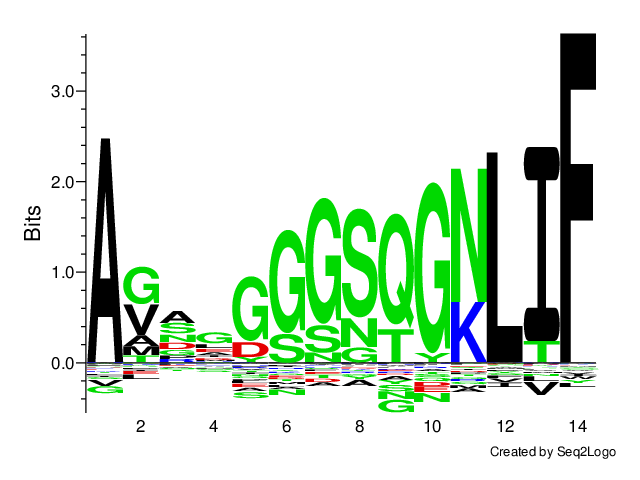
\includegraphics[width=\textwidth]{figures/seq2logo_cd3a_pos.png}
   \caption{}
   \label{fig:logo_cdr3apos} 
\end{subfigure}
\begin{subfigure}[b]{0.45\textwidth}
   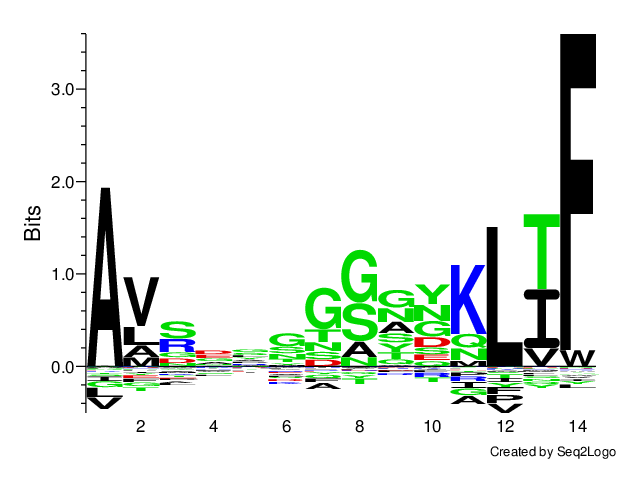
\includegraphics[width=\textwidth]{figures/seq2logo_cd3a_neg.png}
   \caption{}
   \label{fig:logo_cdr3aneg}
\end{subfigure}
\begin{subfigure}[b]{0.45\textwidth}
   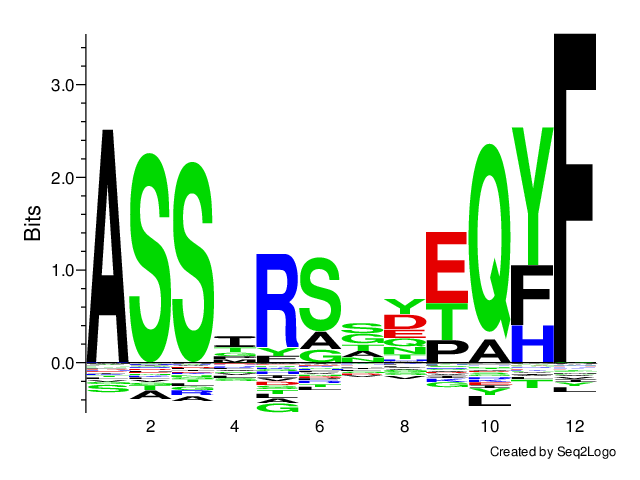
\includegraphics[width=\textwidth]{figures/seq2logo_cdr3b12mer.png}
   \caption{}
   \label{fig:logo_cdr3bpos}
\end{subfigure}
\begin{subfigure}[b]{0.45\textwidth}
   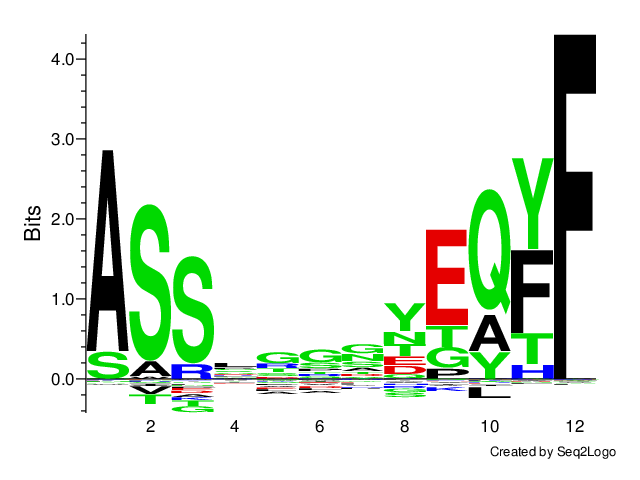
\includegraphics[width=\textwidth]{figures/seq2logo_neg_12mer.png}
   \caption{}
   \label{fig:logo_cdr3bneg}
\end{subfigure}
\caption{Logo plots for CDR3s of \textbf{(a)} positive and \textbf{(b)} negative CDR3{\textalpha} with length 14, and \textbf{(c)} positive and \textbf{(d)} negative CDR3{\textbeta} with lengtg 12. All plots were created using Seq2Logo webserver with 50 as pseudocount weight and no sequence clustering \cite{Thomsen2012Seq2Logo:Depletion}.}
\label{fig:seqlogos}
\end{figure}

\subsection{Word2Vec embeddings capture biochemical features of amino acids}
The Word2Vec model can generate residue-specific embeddings for each amino acid by training the sequence to predict surrounding words. Related amino acids are used in similar contexts within the sequence and therefore predicts the same surrounding residues, and result in similar embeddings. This method is first validated on 20000 proteins randomly sampled from the Swiss-Prot database as described in Section \ref{embedding}. A visualisation of the embedding space reduced to two dimensions by t-SNE can be seen in Figure \ref{fig:emb_prot}.

The plot shows amino acids cluster roughly according to the biochemical properties of the amino acids. Aromatic residues (F, Y and W) are closely related, while the charged residues cluster together (K, R, E and D). The only group not clustering together is polar amino acids. Unique amino acids are not expected to cluster together, as these are not related but generally have distinct properties from all other amino acids.
\begin{figure}
    \centering
    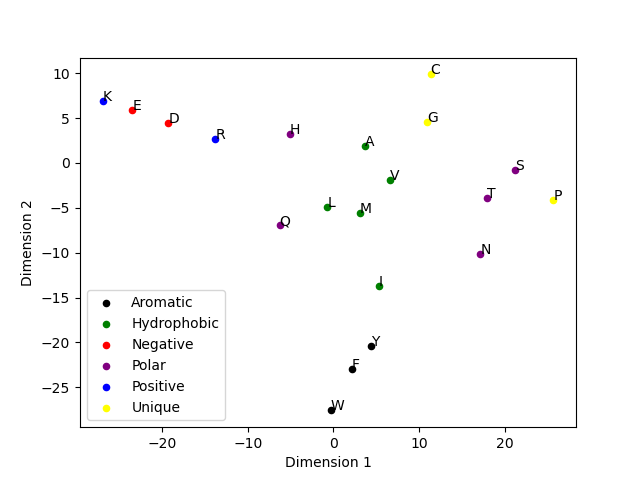
\includegraphics[width=0.65\linewidth]{figures/embedding_proteins.png}
    \caption{t-SNE Visualisation of Word2Vec embeddings trained on random proteins.}
    \label{fig:emb_prot}
\end{figure}

This Word2Vec model only capture rather general aspects of residues. A model trained specifically on CDR3s may generate embeddings allowing to easier separate a positive from a negative TCR. Two models were trained separately for CDR3{\textalpha} and CDR3{\textbeta} sequences. The embeddings are visualised in Figure \ref{fig:emb_cdr3}. Both sets of embeddings do not contain the same clusters as seen in Figure \ref{fig:emb_prot}. The CDR3{\textalpha} still has some similar residues close to one another (F and W, D and E, and hydrophobic residues). In contrast, CDR3{\textbeta} creates seemingly random groups and has histidine as a large outlier.
The embeddings for the CDRs do not seem to capture biochemical features. This does not mean they are of poor quality and bad for predicting TCR-pMHC interactions. They may instead have learned a relationship between amino acids more specific to CDR3s than the general biochemical features.

\begin{figure}[H]
\centering
\begin{subfigure}[b]{0.47\textwidth}
   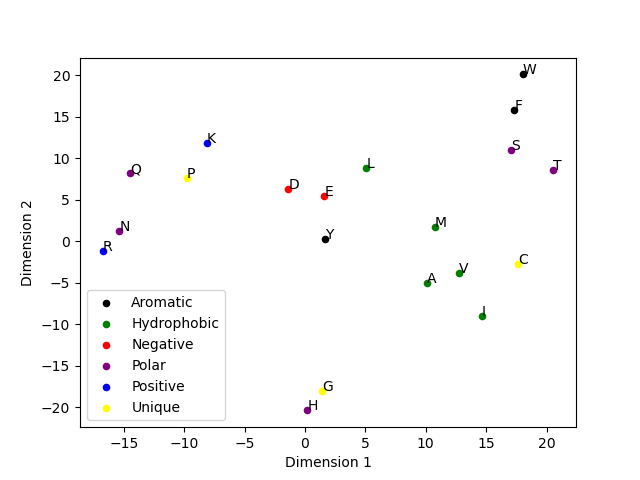
\includegraphics[width=1.125\linewidth]{figures/embedding_cdr3a.png}
   \caption{ CDR3{\textalpha} sequences.}
   \label{fig:emb_cdr3a} 
\end{subfigure}
\begin{subfigure}[b]{0.47\textwidth}
   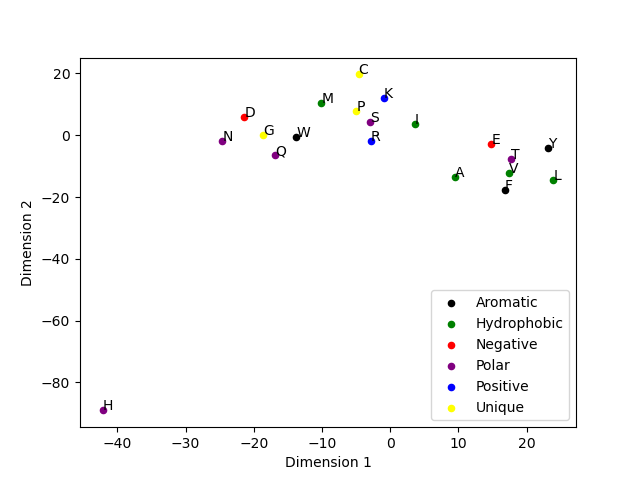
\includegraphics[width=1.125\linewidth]{figures/embedding_cdr3b.png}
   \caption{CDR3{\textbeta} sequences.}
   \label{fig:emb_cdr3b}
\end{subfigure}
\caption{t-SNE Visualisation of Word2Vec embeddings trained on CDR3 sequences.}
\label{fig:emb_cdr3}
\end{figure}

\subsection{Network performances reduces by decreasing redundancy}
The performance of networks depends on the amount of redundancy present in the data. If the data is completely redundant, information leakage between partitions will increase, making predictions on a test set easier. Reducing redundancy also removes data examples, further increasing the difficulty of the prediction problem. The ideal model would be resilient towards redundancy reduction and retain performance as the redundancy is reduced.

The models described in the Methods section were all trained on datasets with decreasing redundancy to investigate which models would be most resilient towards redundancy reduction (Figure \ref{fig:redundancy_compare}). All models were trained on the same data for each selected redundancy value. The CNN model at 0.9 redundancy is the only model not significantly better than the baseline trained on the same dataset (P-value = 0.23 using bootstrapping test with 10000 replications). Every other model is significantly better than the baseline model at all levels of redundancy (P-value < 0.0001 using bootstrapping test with 10000 replications). The LSTM based models significantly outperform the CNN based model at all levels of redundancy (P-value < 0.05 using bootstrapping test with 10000 replications). 

The LSTM based models obtain almost equal performance at the highest level of redundancy. At low amounts of redundancy, the basic LSTM is significantly worse than the more complex models (P-value < 0.0001 using bootstrapping with 10000 replications). Lastly, the effect of incorporating the CDR3 specific embeddings versus a BLOSUM encoding can be seen by comparing the performance of the attLSTM and the Embedded attLSTM (Figure \ref{fig:redundancy_compare}). There was no significant difference between the two (P-value = 0.175), meaning using CDR3 specific embeddings provides no significant performance increase but instead has slightly worse performance than with the more general BLOSUM encoding.

Therefore, the attLSTM outperforms the other model types, and incorporating attention to better focus on important areas outperforms the other types of models tested. Incorporating more advanced embeddings into this model did not give a performance boost, and therefore the more interpretative BLOSUM encoding is preferable to the CDR specific embeddings.

\begin{figure}
    \centering
    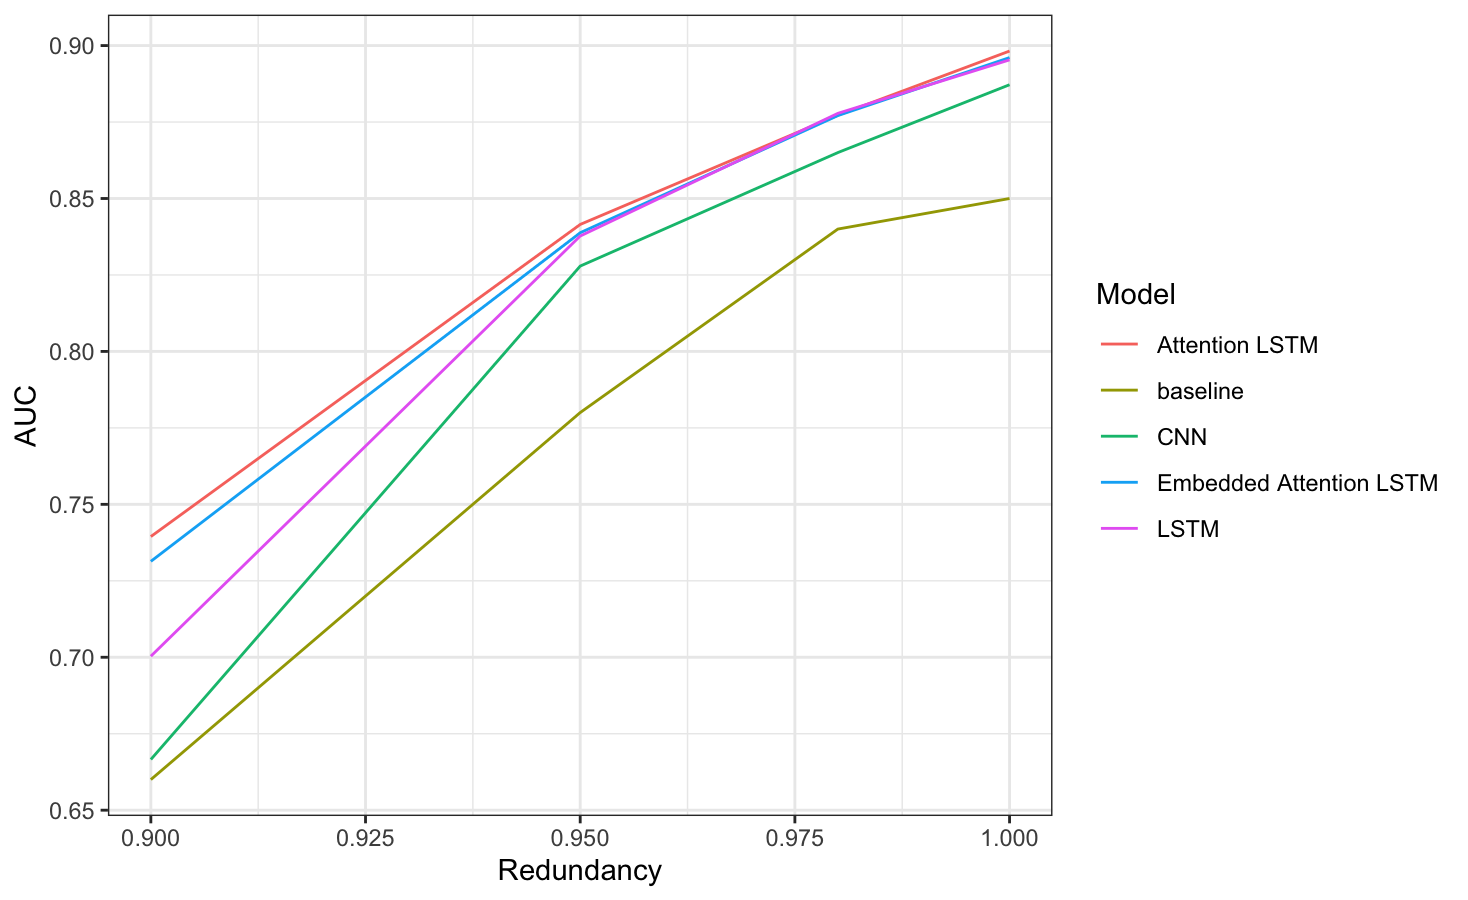
\includegraphics[width=\linewidth]{figures/partition_performance.png}
    \caption{AUCs for the networks tested in this thesis. AUCs were calculated using nested crossvalidation.}
    \label{fig:redundancy_compare}
\end{figure}

\subsection{attLSTM Network Performances}

The attLSTM outperformed the other model architectures at low redundancy and was equivalent to the base LSTM at high redundancies and obtained an AUC score of 0.88 for the full dataset. To further describe the performance of the attLSTM model, the per peptide performances were investigated (Figure \ref{fig:performance_pr_pep}). As previously shown, the performance drops as redundancy is reduced. However, only a few peptides drive the total performance. Only the peptides with a high number of observations obtain performance beyond random (AUC of 0.5). The model achieves good performance on both the GIL and GLC peptides (AUC of 0.91 and 0.84) and even retains some performance at high levels of redundancy (AUC of 0.76 and 0.69). The NLV achieves some performance at high redundancy (AUC of 0.64), but the performance becomes random when the redundancy is reduced.

The remaining peptides generally obtain random or worse than random performance. The FLYALALLL peptide is an exception and obtains high performance with only a few positive peptides. This is because the sequence dissimilarity for positive and negative sequences is large, meaning distinguishing between positives and negatives is simpler for the model \cite{Montemurro2021NetTCR-2.0Data}.

While the model obtains great performance, this performance is restricted to only a few peptides. The trend is generally that peptides with a high number of positive sequences obtain a better performance. Therefore, obtaining more data for a larger number of peptides is likely required to make the model better at predicting the peptides with limited data.

\begin{figure}
    \centering
    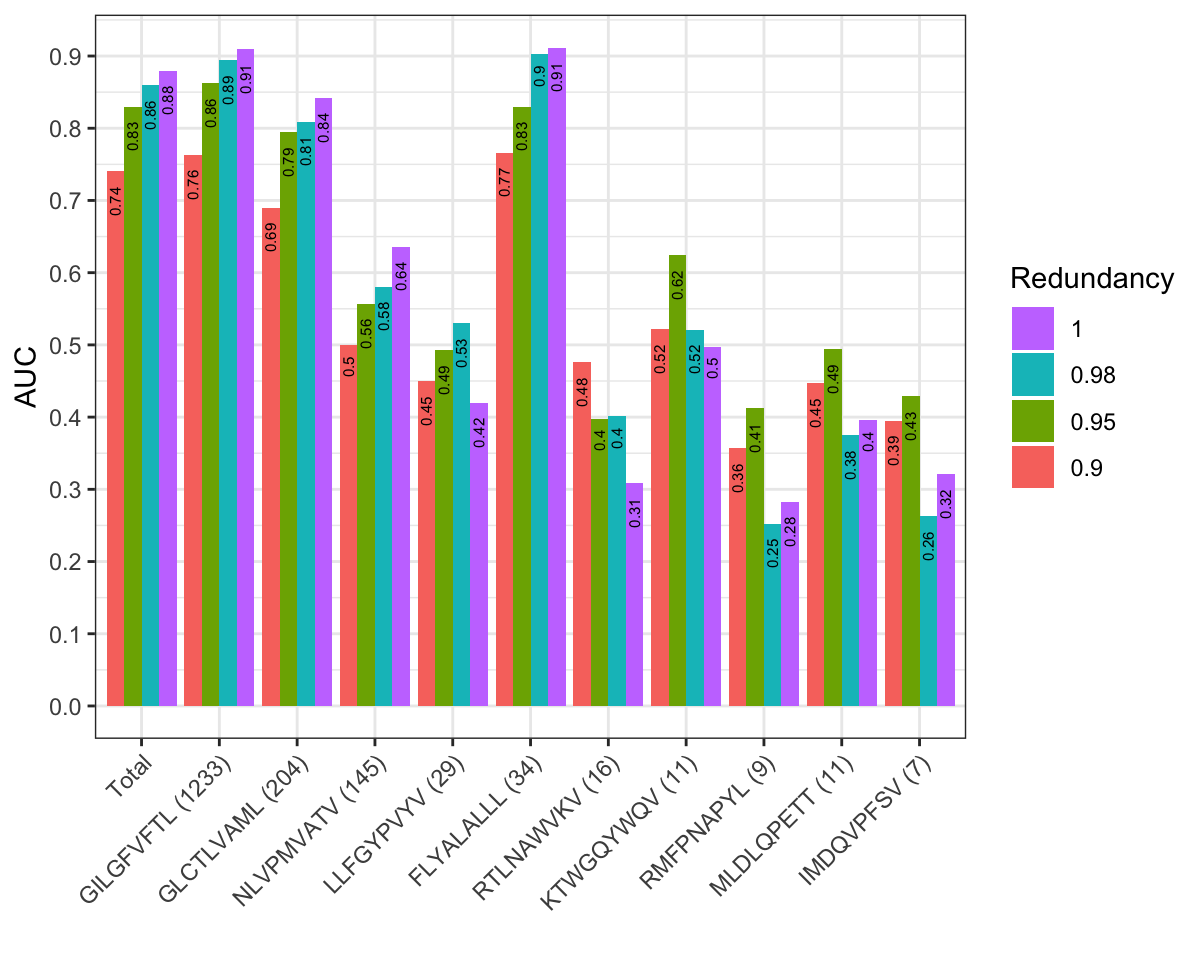
\includegraphics[width=\linewidth]{figures/peptide_performance.png}
    \caption{AUCs for each peptide, at each level of redundancy. AUCs were calculated using nested crossvalidation. Number of positive TCRs in the complete dataset is shown in parenthesis.}
    \label{fig:performance_pr_pep}
\end{figure}

\subsubsection{Swapped negative performance versus 10x negative performance}

The swapped negatives were created to ensure the model learns that TCRs only bind a specific peptide and not all possible peptides. The model could have issues with discriminating between the swapped and positives, leading to low performance on swapped observations. The AUCs for the attLSTM were calculated using all observations, excluding 10x negatives and excluding the swapped observations (Figure \ref{fig:swap_vs_10x}a). The swapped negatives seem easier for the model to predict, which is counterintuitive considering these TCRs resemble positive TCRs more than a 10x negative.

The output scores for each type of negative are also different (Figure \ref{fig:swap_vs_10x}b). The swapped negatives generally obtain lower scores than the 10x negatives. Swapped negatives could be easier to predict, as most of the swapped were originally GIL positive. Since the model can pick out GIL positive TCRs, it may have learned that if this type of TCR is observed with another peptide than GIL, it is negative. Additionally, positive observations have high scores for peptides with many observations but low scores for peptides with limited data (Figure \ref{fig:performance_pr_pep}), again supporting that the model only learns to recognize positive TCRs for a small number of peptides.

\begin{figure}
    \centering
    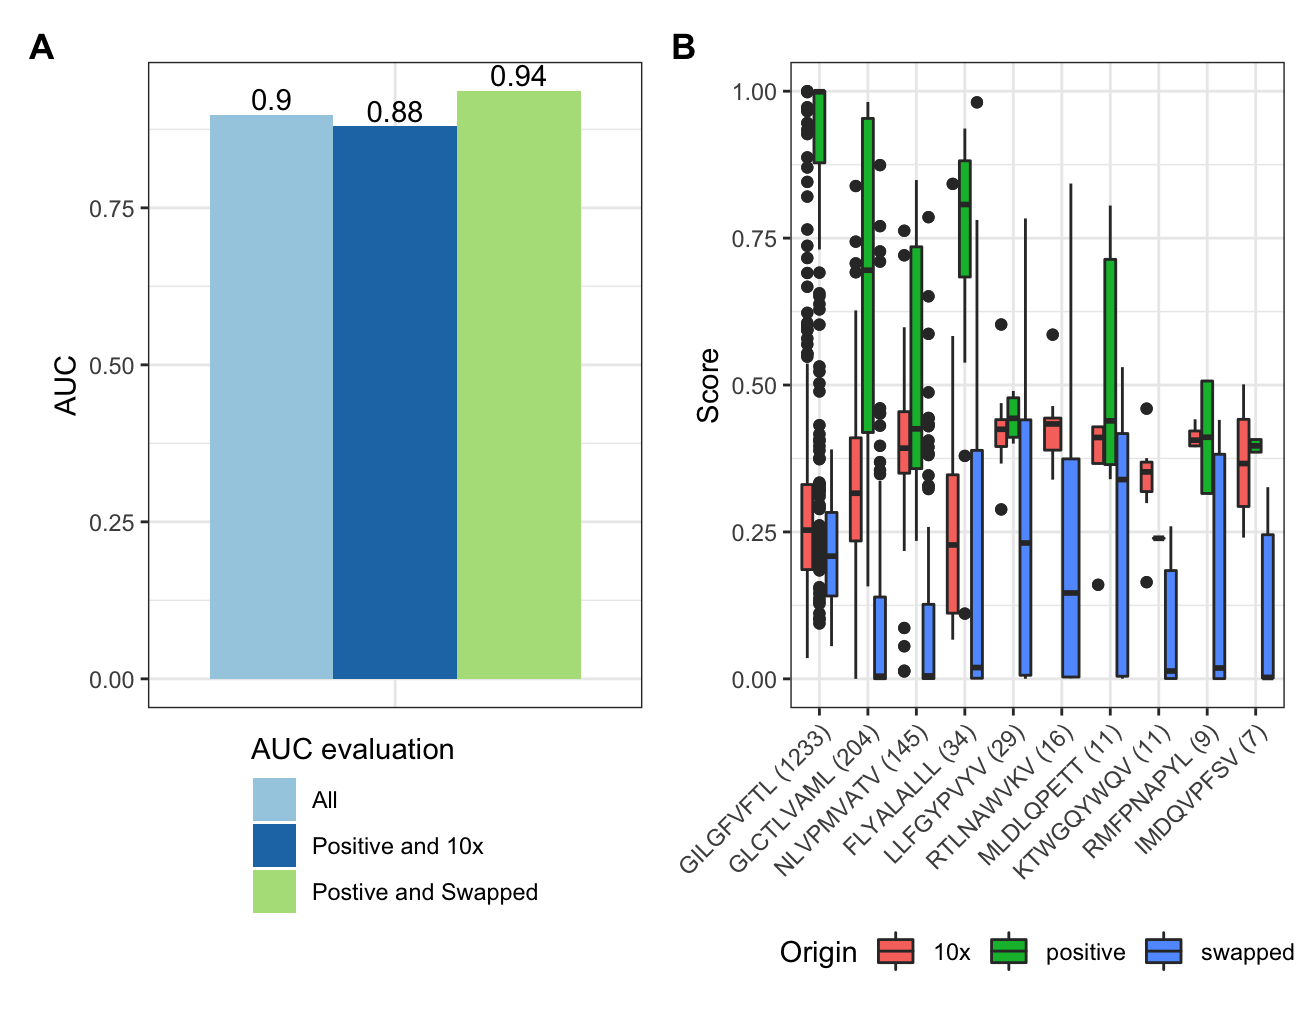
\includegraphics[width=\linewidth]{figures/swapped_10x_performances.png}
    \caption{\textbf{(A)} AUCs evaluated on either all data, excluding swapped negatives or excluding 10x negatives.\textbf{(B)} output scores for each type of observation. Scores were obtained from a held out partition. Number of positive observations for each peptide is denoted in parenthesis.}
    \label{fig:swap_vs_10x}
\end{figure}


\subsection{Cross peptide information boosts performance when data is limited}
The previously trained models were all pan-specific models, where all peptides were trained and predicted using the same model. In this way, information on all peptides is available for the entire training, and the model can be used to predict all peptides. A peptide-specific model might achieve better performance for individual peptides, considering the model would only have to learn what makes TCRs bind to a single peptide. However, if there is any information, such as binding positions, which are universal for TCRs regardless of peptide specificity a pan-specific model could be better on individual peptides as well.

Th best way of incorporating new peptides were tested by making three types of models. A pan-specific model, which is the general model used in this thesis and is trained on data from all available peptides. The peptide-specific model, which is used to test if there are any benefits from adding data from other peptides, or if a model works better trained on data only from the specific peptide. The last model is considered as a compromise between the two. First a pan-specific model is trained without the peptide in question, similarly to a leave peptide out setting. This model is then used to initialize a peptide-specific model for the peptide left out (i.e. a pan-specific model is trained using all peptides except GIL, and then used to initialize a peptide-specific GIL model). These are the three models used for Figure \ref{fig:subsampling_models}.

Hopefully, the pre-trained peptide-specific model could learn some of the universal aspects of TCR binding from the pan-specific model and then the specifics of that specific peptide, resulting in the best of both models. The pre-trained peptide-specific model simulates the situation where a general pan-specific model could be trained and then fine-tuned to predict a new peptide not currently in the pan-specific model using a small number of observations for this peptide.

The three models mentioned above were trained on a decreasing amount of observations for the peptide in question. All data from other peptides were used for training the pan-specific and for the pre-training of the pre-trained peptide-specific model. This means we observe the drop in performance directly as a consequence of the number of observations for this peptide in the training set, as opposed to Figure \ref{fig:redundancy_compare}, where all observations were subsampled.

Figure \ref{fig:subsampling_models} shows how the performance of a specific peptide is affected by reducing the number of observations for that peptide in the training set.  For all models, the performance drops as the number of observations are reduced. The performance on GIL is almost constant with many positives, and all models seem to drop performance around 100-150 positive observations. This drop is not as clear for the other peptides, but the number of positives is also much lower, and the performance drop might not be visible in these plots.

Comparing the individual models on the GIL peptide, the peptide-specific and pan-specific models significantly outperform the pre-trained peptide-specific model (P-value < 0.05 using bootstrapping test with 10000 replications) when the number of positives is high (724 and 550). At a low number of positives (15 and 35), the pre-trained peptide-specific and pan-specific model significantly outperforms the peptide-specific model (P-value < 0.05 using bootstrapping test with 10000 replications). Therefore, the peptide-specific model seems best for peptides with a high number of positives. In contrast, the pan-specific model (and the pre-trained peptide-specific model) is better when few observations are available for that peptide. At the same time, the peptide-specific models (both the pre-trained and not pre-trained) are more unstable with a low number of observations and could yield spurious predictions. 

For the GLC, there is a trend for the two peptide-specific models to have a slight edge compared to the pan-specific models, but no differences were significant. Here the number of observations is also drastically lower, which might explain why the trend from the GIL model is not observed. Lastly, the NLV models have an even lower amount of observations. However, the pre-trained peptide-specific and pan-specific models are significantly better than the peptide-specific model at all numbers of positives, except for 72 positives (P values < 0.05 with bootstrapping test using 10000 replications). This again supports that both the pre-trained peptide-specific and the pan-specific model are better with fewer observations than a peptide-specific model.

\begin{figure}
    \centering
    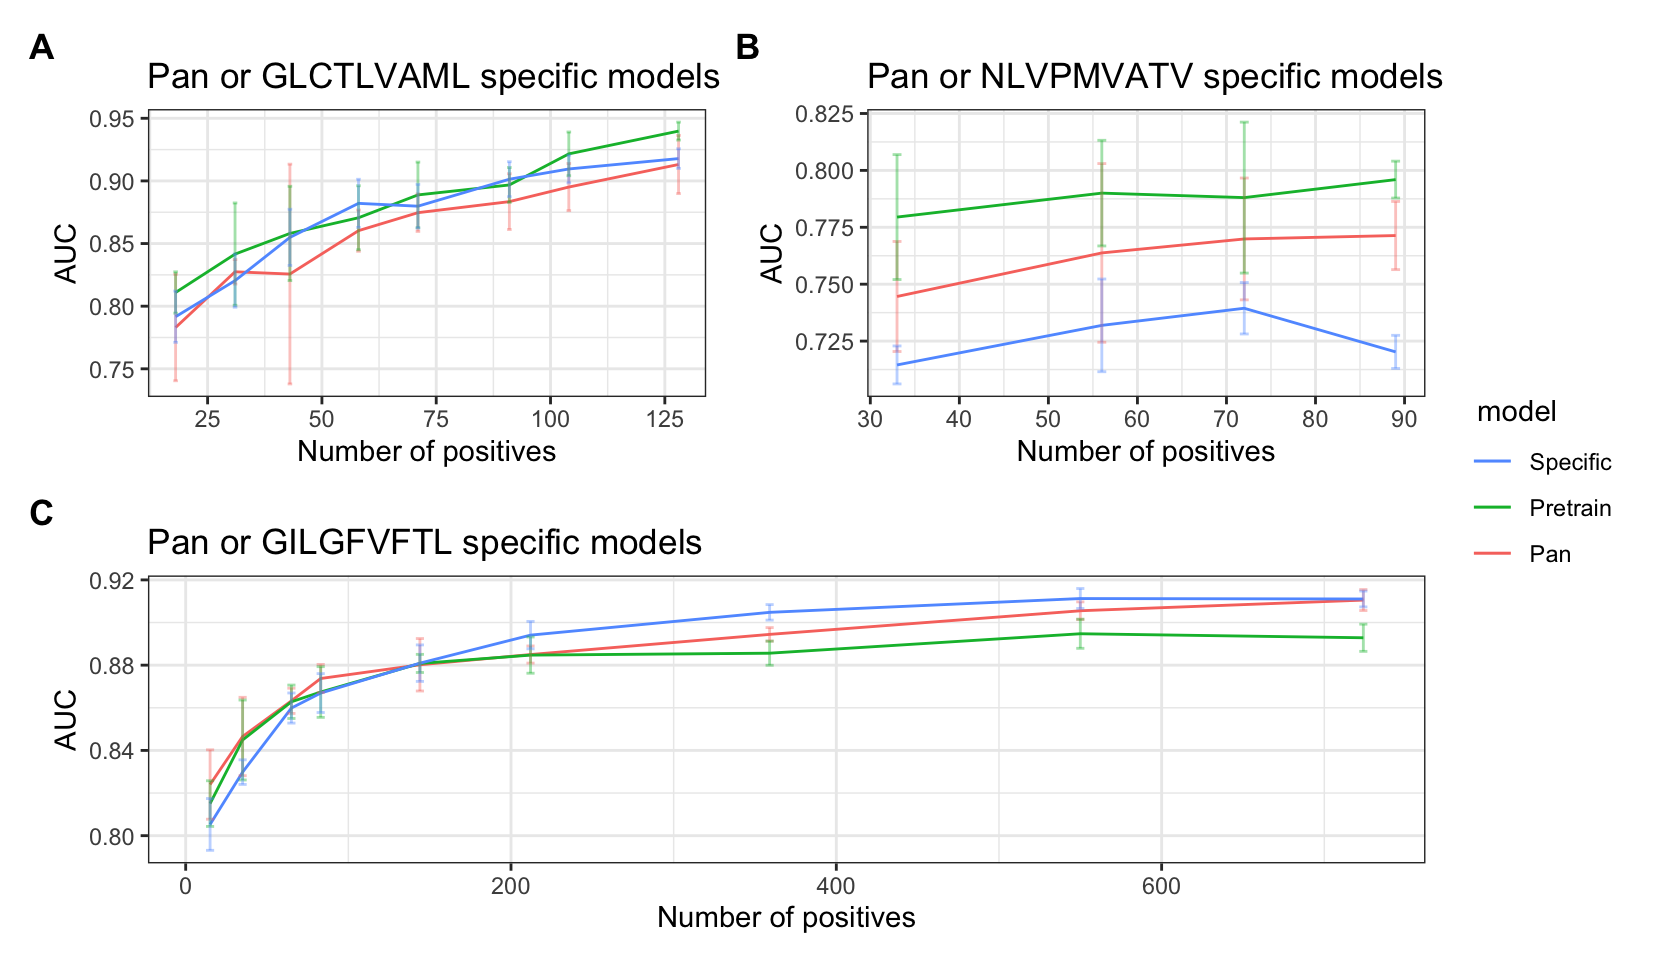
\includegraphics[width=\linewidth]{figures/subsampling_peptide_models.png}
    \caption{Model performance as a function of the number of positives in the dataset for the three most prevalent peptides in the data. For each of the three peptides, three types of models (peptide specific, pan-specific specific and pre-trained peptide specifc) were trained on varying amounts of data for the specific peptide. The pan-specific model contained a constant amount of data for all other peptides and only varied the peptide in question. The pre-trained peptide specific model was initialized from a pre-trained pan-specific model (trained on the same data as the pan, but without the peptide in question). Lastly the peptide specific model was only trained on the peptide in question. AUCs were calculated from observations with same peptide specificities (\textbf{A}) GLC, (\textbf{B}) NLV or (\textbf{C}) GIL taken from a constant held out partition which was not subsampled. Each model was trained 5 times, average AUC and standard deviation is reported.}
    \label{fig:subsampling_models}
\end{figure}

\subsection{Specificity Predictions}
Up till now, the models have only been evaluated on how good they are at predicting whether a given TCR is positive or negative for a given peptide. However, an ideal model should also be able to distinguish between what peptide a given TCR would be bind. In theory, a pan-specific model should be better at this than a peptide-specific model since it has seen information about other peptides. However, Using the pre-trained peptide-specific model, the model has previously seen information about other peptides during pre-training and could perhaps remember this when predicting specificity. A test set was created using all positives from a held-out test set and 10 swapped negatives for each of these positive TCRs. Therefore, the test set has 11 observations for each unique TCR, but only one of which is positive. An ideal model should give the positive a high score, while the swapped should be recognized as negative and given a low score.

An AUC was calculated for each unique TCR using the predictions from each observation. If the positive observation had the highest prediction score, the AUC would be one and zero if all the swapped observations achieved higher scores than the positive. The pan-specific model generally achieves better performance in predicting specificity than the pre-trained peptide-specific model (Figure \ref{fig:specificity_performance}A). As the pan-specific model is trained on all peptides and contains swapped negatives, the model is forced to learn what makes a TCR positive towards GIL, whereas the peptide-specific model only learns what makes a TCR positive. 

AUCs for GIL TCRs show that the pan-specific model can almost completely predict the correct peptide, while the pre-trained peptide-specific model tends to predict the correct peptide most of the time, but not as often as the pan-specific model. The difference is even clearer for the GLC peptide, where only a few TCRs are correctly identified as GLC positive for the peptide-specific model. Lastly, the NLV specific TCRs are rarely predicted correctly using either model, meaning specificity predictions are only really feasible for peptides with a high number of TCRs.

The difference between the two models can be found in their distributions of scores (Figure \ref{fig:specificity_performance}B). The pan-specific model has a much better separation in GIL and GLC scores than the pre-trained peptide-specific model, where the scores seem to distribute almost identically. This supports the idea that the pan-specific model is better at specificity predictions, as it learns to distinguish between peptides. In contrast, a peptide-specific model is not trained with this in mind and only learns what distinguishes a positive and negative TCR for that specific peptide. Therefore, even with pre-training on other peptides, the pre-trained peptide-specific model cannot compete with a pan-specific model when it comes to specificity predictions.

\begin{figure}
    \centering
    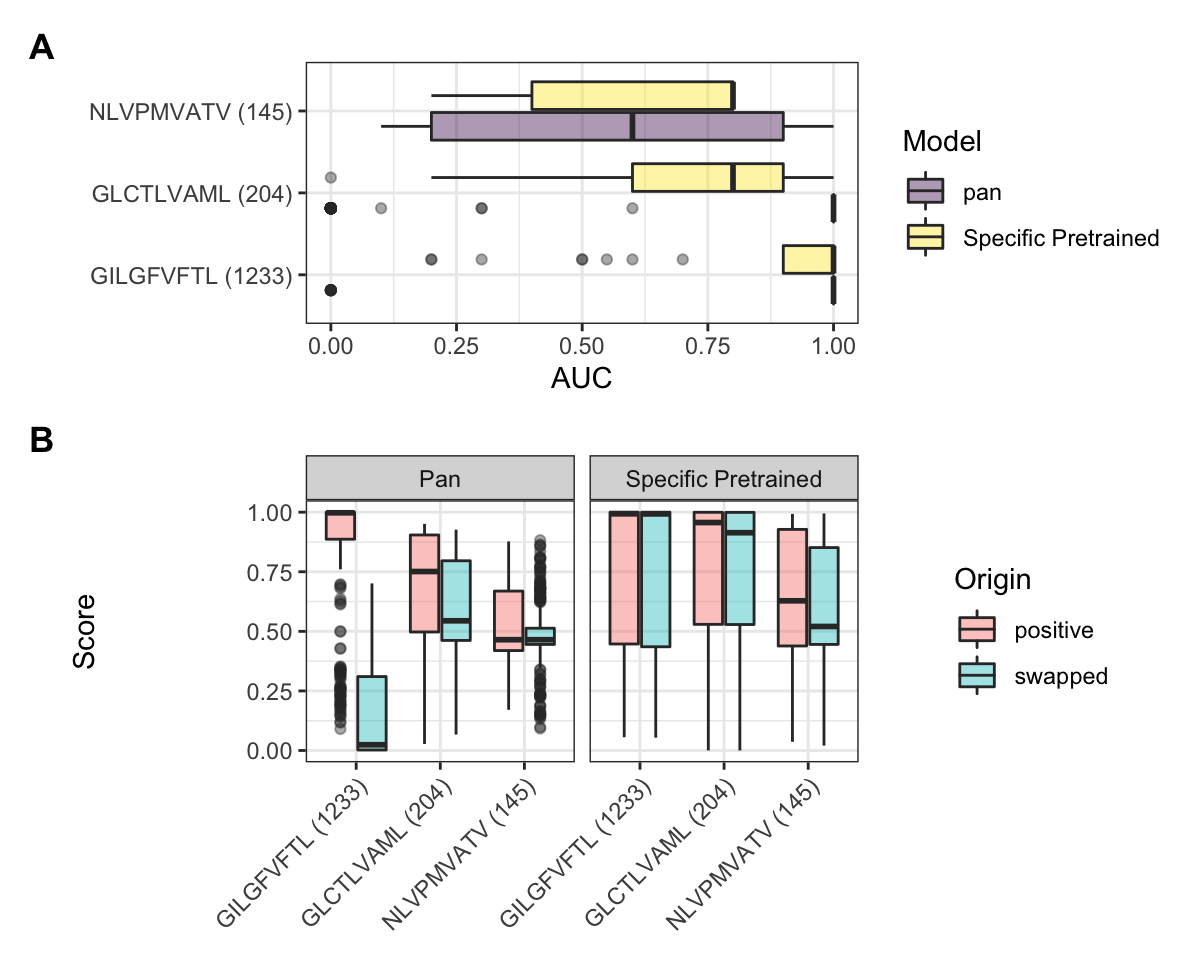
\includegraphics[width=\linewidth]{figures/pretrain_specificity.png}
    \caption{TCR specificity predictions for the 3 most prevalent peptides in the dataset. Number of positives in the dataset is noted in parenthesis. The trained models were evaluated on a test set with all positives from a held out test set, along with 10 randomly sampled swapped negatives created from each positive in the held out set. \textbf{(A)} AUCs evaluated for each unique TCR in the testset. \textbf{(B)} output scores for binding generated for the testset.}
    \label{fig:specificity_performance}
\end{figure}






